\documentclass[12pt,a4paper,titlepage]{report}

% Document Info
%
\newcommand\AcademicTitle{Dynamic Performance Framework}
\newcommand\CommericalTitle{Iris}
\newcommand\Author{Dean Gaffney}
\newcommand\StudentID{20067423}
\newcommand\Date{December 2017}
\newcommand\Report{Status Report (Semester 2)}
\newcommand\Reader{Supervisor: Dr.~Kieran Murphy}
\newcommand\SecondReader{Second Reader: David Drohan}

\usepackage{fyp_document}

\newcommand*{\mybox}[2]{\colorbox{#1!30}{\parbox{.98\linewidth}{#2}}}
\newcommand{\q}[1]{``#1''}

\crefname{paragraph}{paragraph}{paragraphs}
\Crefname{paragraph}{Paragraph}{Paragraphs}

\begin{document}

\pagenumbering{roman}

% title page as per Ian's spec
\thispagestyle{empty}
\begin{center}
\mbox{}\vfill
{\fontsize{18pt}{20pt}\selectfont \bfseries \AcademicTitle}
\vfill
{\fontsize{14pt}{20pt}\selectfont \bfseries\itshape \CommericalTitle}
\vfill
{\fontsize{12pt}{20pt}\selectfont \bfseries \Report}
\vfill
{\fontsize{14pt}{20pt}\selectfont \bfseries \Author}
\vfill
{\fontsize{14pt}{20pt}\selectfont \bfseries \StudentID\ Panel 3}
\vfill
{\fontsize{14pt}{20pt}\selectfont \bfseries \Reader}
\vfill
% {\fontsize{14pt}{20pt}\selectfont \bfseries \SecondReader}
\vfill
{\fontsize{14pt}{20pt}\selectfont \bfseries BSc (Hons) in Entertainment Systems}
\vfill
\end{center}
\clearpage

\tableofcontents
\listoftables
\listoffigures

% start of main matter
\clearpage
\pagenumbering{arabic}
\setcounter{page}{1}

\chapter{Abstract}

The aim of this project is to design a full implementation of a system for application performance monitoring. The proposed system, has the working title,  Iris.

Iris provides users with a dynamic performance framework which allows users to fully customise and centralise their application performance monitoring. This is achieved through a web interface where a user specifies a schema for a specific application they wish to monitor. Once a schema has been set up, a REST endpoint is generated for the application. This endpoint allows a user to send their monitoring data from their desired application to the framework in the form of JSON (matching the specified schema). Iris also contains features which allow a user to monitor and analyse incoming data, using an intelligent, fully customisable graph and dashboard builder. Iris then visualises any received data in real time to appropriate dashboards using websockets.

\chapter{Introduction}

\section{Motivation for Iris}
The following section is identical to the Motivation for Iris section in the Semester 1 report. It has been added here for convenience.

The motivation for this project comes from database and system performance issues that Onaware\footnote{Onaware is an international company that specialises in IAM (Identity and Access Management) and has offices with 20 staff in Waterford. More information on Onaware can be found at \url{https://onaware.com}.} has experienced in recent projects. It is often the case that they must deal with large amounts of identity data being aggregated into a third party system called `IIQ'.

Onaware has faced major issues with aggregating data in the past, in some cases it was taking up to five days, and sometimes aggregations would fail halfway through meaning aggregations would have to be restarted; due to the amount of software involved it is hard to pinpoint what software is causing the issue.

In one such instance of aggregating data issues several attempts were made to rectify the performance issue such as optimising sql queries, increasing ram, multi threading tasks and increasing disk space, none of which worked. Due to the performance issue the IIQ instance became unusable so debugging the issue was not possible from inside the application and log files became so big that text editors would crash when trying to open them. In this case the issue turned out to be a customer putting size constraints on the database storing the aggregated data. While monitoring would not prevent such a mistake it would have reduced the time needed to locate the issue.

In response to difficulties in identifying performance issues Onaware have tried to monitor specific application elements. The aim at the time was to try and combine SQL, JVM and Operating System scripts to track the performance of the tools, however this approach is not very scalable and it would need to be reconfigured for future projects.

Iris is an attempt to solve this problem. Iris allows a user create a new application monitor with little effort using a web interface, give the user a REST endpoint specific to the application for their scripts to target their data and allow a user to monitor the data in real time using graphs and dashboards. The aim is to make the framework as flexible as possible and not specific to the issue Onaware faced, meaning a user can monitor any data they want from any application they want all they must do is send their data to a REST endpoint.

\begin{figure}[H]
\begin{tcolorbox}
\begin{center}
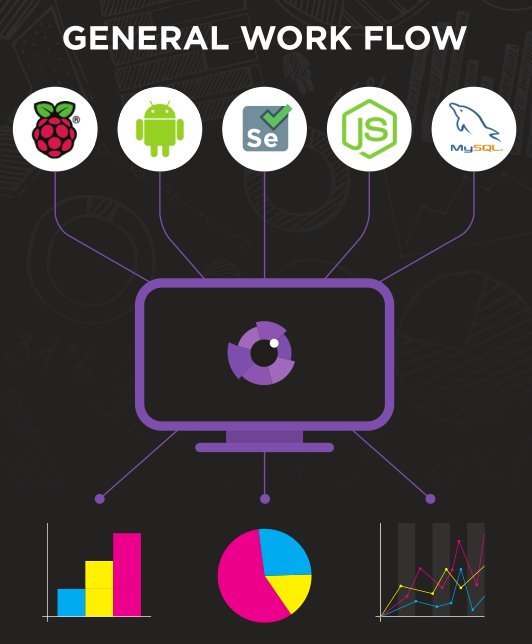
\includegraphics[width=\textwidth,height=\textheight,keepaspectratio]{iris-general-workflow}
\end{center}
\end{tcolorbox}
\caption{High level view of the Iris system.}
\end{figure}

\begin{figure}[H]
\begin{tcolorbox}
\begin{center}
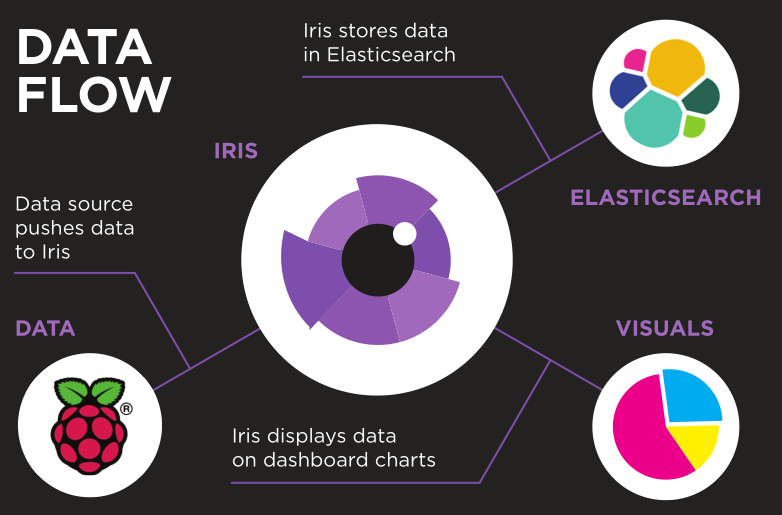
\includegraphics[width=\textwidth,height=\textheight,keepaspectratio]{iris-data-flow}
\end{center}
\end{tcolorbox}
\caption{High level view of the data flow in Iris.}
\end{figure}

Users of Iris will consist of Onaware developers who will be monitoring IAM (Identity Access Management) project data and generic tools which may be released to clients at a later time.

\section{Features List}
The features of Iris follow closely to that of Kibana. Iris adds some extra features which Kibana does not support, these are as follows:
\begin{itemize}
    \item Real-Time Monitoring
    \item Elasticsearch Aggregation Builder
    \item Automatic Elasticsearch Mapping
    \item Elasticsearch Aggregation Playground
    \item Centralised Data Transformation
    \item User Specific Dashboards
    \item Dashboard Builder
    \item Dashboard Revision History
    \item Unique Application Endpoint Generation
\end{itemize}
\subsection{Types of Data}
Iris currently supports several types of data, they are as follows:
\begin{itemize}
    \item Numerical
    \item Categorical
    \item Raw
\end{itemize}

Support for the different types of data are demonstrated on dashboard charts in \cref{s:implementation:datasource}.

\chapter{Implementation}
During Semester 1 a number of implementations were designed and tested. As a result the implementation described in the Semester 1 report required no further changes in this Semester. Hence, this section is fundamentally unchanged from that in the Semester 1 report and the summary of the implementation design is reproduced here with some minor modifications. The subsections dealing with components implemented in Semester 2 is fundamentally new. \Cref{table:component:completion} lists the components and when they were completed. 
\begin{table}[H]
\centering
\small
\setlength\tabcolsep{6pt}
 \begin{tabular}{|c|c|c|}
 \hline
 Component & Prototyped & Implementation\\
 \hline\hline
 Core Framework/Services & Semester 1 & Semester 1\\ 
 \hline
 Schemas & Semester 1 & Semester 2\\ 
 \hline
 Dashboard & Semester 1 & Semester 2\\ 
 \hline
 Data Sources & Semester 2 & Semester 2\\ 
 \hline
 Security & Semester 1 & Semester 2\\ 
 \hline
\end{tabular}
\caption{Summary of component completion.}
\label{table:component:completion}
\end{table}

\section{Core Framework/Services}
In the Semester 1 report the design of Iris is described. Due to the testing of the designs in the first Semester the final design needed no further modifications this Semester. Hence the description of Iris given here follows closely that given in report 1.

\subsection{Description}
Iris acts as a web interface for a user to create an application monitor and allow the user to query and create personalised dashboards of their data through the use of Elasticsearch. A user may setup an application schema definition within Iris that matches the data they wish to monitor, a schema consists of field names and corresponding data types specific to the application. Iris uses the schema to know what data to expect from the user. Once a schema is in place, Iris generates a unique endpoint associated with the schema, this unique endpoint is made available to the user as a means of sending data to Iris. Data sent to the schema endpoint is in JSON format which conforms to the schema definition created by the user in Iris.
\begin{figure}[H]
\begin{tcolorbox}
A user creates an application monitor for an SQL database, they may create a schema like the following:
\begin{minted}{yaml}
Schema Name: "SQL Monitor"
Schema Fields:
    -field name: "writeSpeed"
     fieldType: "double"
    -field name: "tableName"
     fieldType: "String"
\end{minted}
Iris then expects a json object to come back in the form:
\begin{minted}{json}
{
	"writeSpeed": 3000,
	"tableName":  "students"
}
\end{minted}
\end{tcolorbox}
\caption{Example schema created for Iris.}
\end{figure}

Iris takes the users data and creates data mappings \parencite{Elastic.co.Mapping} inside Elasticsearch, as well as inserts any incoming data into the correct Elasticsearch index~\parencite{Elastic.co.Basic}. With a schema in place a user can route their data through Iris; turning Iris into a centralised area for monitoring application performance data. With Iris being the centralised location to route and view your data a user can write a data transformation script for incoming data. The advantage of this is that it can help reduce the need for applications being redeployed to transform data.

\begin{figure}[H]
\begin{tcolorbox}

The user releases their application, and it is downloaded by 500 people. This data is now being sent from 500 instances of this application. To make any change to this data the developer must add in their desired field and and redeploy the app, those 500 users would then need to download an update for the application in order for it to take effect. The original JSON object passing through Iris looks like the following:
\begin{minted}{json}
{
	"firstName": "Dean",
	"lastName":  "Gaffney"
}
\end{minted}

In this example let's say the developer prefers to have the data mapped to a field called \q{fullName} which is all lowercase, the developer wants to avoid having to redeploy the app for one single field, instead the developer goes to Iris and applies a script to the schema. By running the script on incoming data the developer has made their desired change in a central location with no redeploys. The data may look like this after the developer has applied the script to the data:
\begin{minted}{json}
{
	"firstName": "Dean",
	"lastName":  "Gaffney",
	"fullName":  "Dean Gaffney"
}
\end{minted}
\end{tcolorbox}
\caption{Iris transforming data.}
\end{figure}

To aid performance monitoring, Iris allows users to create personalised dashboards where they can create charts from their data and place them in the dashboard. This allows each user to have their own set of visualised data relative to them. To help a user see their data and charts rapidly an Elasticsearch aggregation~\parencite{Elastic.co.Aggregations} playground is available in order to allow a user to test their data and get results back immediately, this will help a user to plan their dashboard charts before setting them up. The playground also allows a user to chain several aggregations together which allows them to create complex queries without having to have any prior knowledge of how Elasticsearch works.

 
\subsection{Schemas}
Schemas in Iris have not changed from Semester 1 in terms of their design, they are still used as a representation of a data source in Iris which is created by the user. However there were some improvements made on both the front and backend of Iris to make the creation and interaction of agents with schemas easier for the user. These improvements will be discussed in the following sections.
\subsubsection{Frontend}
This section will discuss the improvements made to the frontend of Iris in regards to the Schema section.

\paragraph{Schema Fields}
Iris now displays the Schema Fields in a table fashion and presents the user with the name and data types of all the fields in the schema.
\begin{figure}[H]
\begin{tcolorbox}
\begin{center}
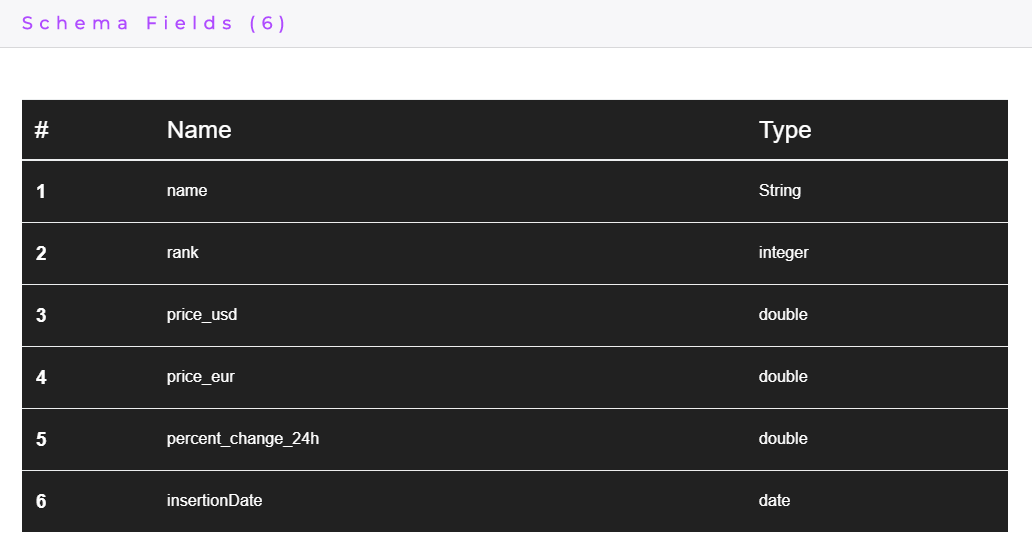
\includegraphics[width=\textwidth,height=\textheight,keepaspectratio]{iris-schema-fields}
\end{center}
A screenshot of the schema fields belonging to the Node.js schema in Iris.
\end{tcolorbox}
\caption{Node.js schema fields in Iris.}
\end{figure}

\paragraph{Data Source Endpoint}
Iris now displays the unique endpoint associated with a data source when you click on the schema in Iris. This allows a user to see what address their data source must use as well as test out the endpoint before committing to writing a data source that uses the endpoint.

\begin{figure}[H]
\begin{tcolorbox}
\begin{center}
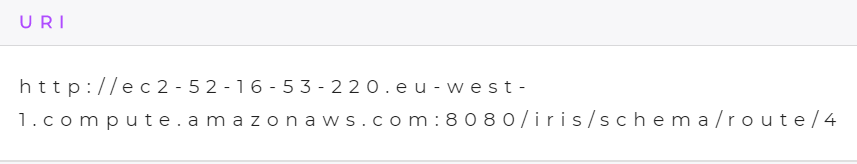
\includegraphics[width=\textwidth,height=\textheight,keepaspectratio]{iris-schema-endpoint}
\end{center}
A screenshot of the MySQL data source endpoint in Iris.
\end{tcolorbox}
\caption{MySQL data source endpoint in Iris.}
\end{figure}

\paragraph{Expected JSON}
Iris now displays the expected JSON object from the data source as well as the data types that are associated with each key in the object. This aids users when they are writing code for data sources as they can refer back to Iris to see what format their JSON object needs to conform to.

\begin{figure}[H]
\begin{tcolorbox}
\begin{center}
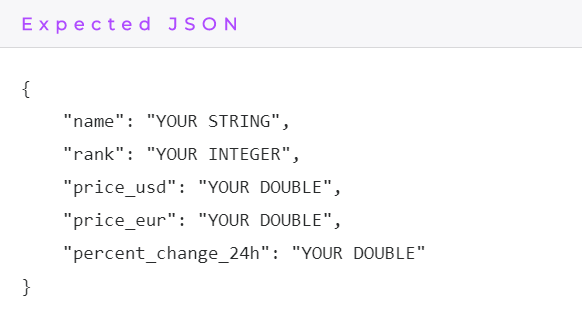
\includegraphics[width=\textwidth,height=\textheight,keepaspectratio]{iris-schema-expected-json}
\end{center}
A screenshot of the expected JSON for the Raspberry Pi data source in Iris.
\end{tcolorbox}
\caption{Expected JSON for Raspberry Pi data source.}
\end{figure}

\paragraph{Transformation/Rule Script Editor}
Due to Iris' ability to allow users to write transformation scripts that run on incoming data which is discussed in \cref{para:rule:executor:backend}, a code editor was embedded into Iris. The code editor being used is the `Ace' code editor with Groovy syntax highlighting which aims to aid the user in writing small transformation scripts.

\begin{figure}[H]
\begin{tcolorbox}
\begin{center}
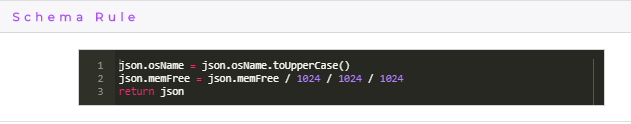
\includegraphics[width=\textwidth,height=\textheight,keepaspectratio]{node-transformation-script}
\end{center}
A screenshot of the Transformation Rule script on the Node.js schema written using the `Ace' code editor.
\end{tcolorbox}
\caption{Node.js transformation rule script.}
\label{fig:rule:executor}
\end{figure}

More information on the `Ace' code editor can be found here \url{https://ace.c9.io/}

\paragraph{Schema Overview}
The following section ties together the previous front end sections and shows what an entire schema looks like inside Iris in a single image.

\begin{figure}[H]
\begin{tcolorbox}
\begin{center}
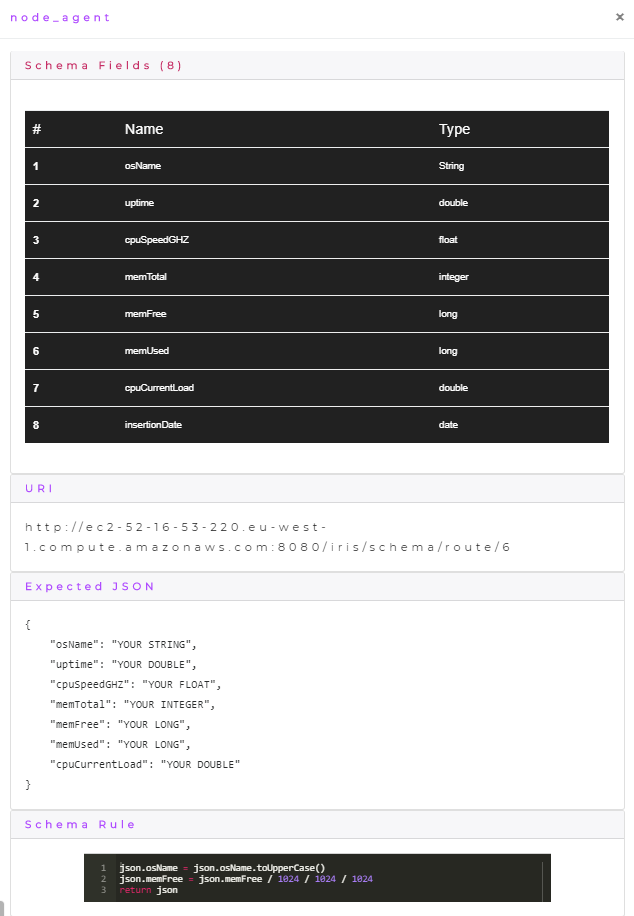
\includegraphics[width=0.8\textwidth,height=0.8\textheight]{iris-node-schema}
\end{center}
A screenshot of the Node.js agent schema in Iris.
\end{tcolorbox}
\caption{Node.js agent schema in Iris.}
\end{figure}

\subsubsection{Backend}
This section will discuss the improvements made to the backend of Iris in regards to the Schema section.

\paragraph{Transformation/Rule Script Execution}
\label{para:rule:executor:backend}
In the Semester 1 report it was briefly discussed that Iris would allow users to write their own scripts inside Iris to allow a user to modify incoming data, which would avoid a user having to redeploy their data source to make a small change to the data they are pushing ot Iris. A user would mainly use this feature for formatting dates, strings and numerical values before it is inserted into Elasticsearch and rendered on the user's dashboard. This feature is now fully supported in Iris and an image of a transformation script can be found in \cref{fig:rule:executor}

\paragraph{Data Source Endpoint Retrieval}
Iris now accepts `POST' requests to the endpoint \url{$SERVER_BASE/schema/getAgentUrl} and expects a JSON body with the request like the following:

\begin{figure}[H]
\begin{tcolorbox}
\begin{minted}{json}
{
    "name": "someSchemaName"
}
\end{minted}
\end{tcolorbox}
\caption{SchemaController `getAgentUrl' endpoint JSON payload.}
\end{figure}
Assuming the user is authenticated, Iris will look for a Schema matching this name and return the unique endpoint for this schema. The advantage of this is that a user may create a schema and not be satisfied with it. The user may then decide to delete the schema and create a new schema using the same name with extra attributes attached to it. The issue here is that Iris will give the new schema a new url different from the previous schema. This now means a user must go back to their agent code and change a hardcoded url to a new url and then redeploy the agent. However if a user writes their code to take advantage of the `getAgentUrl' endpoint in Iris, they will be able to dynamically obtain a new unique endpoint for the new schema as long as the schema name stays the same. This means there is no need to redeploy the agent with a new url as it is obtained dynamically from Iris.

\begin{figure}[H]
\begin{tcolorbox}
\begin{center}
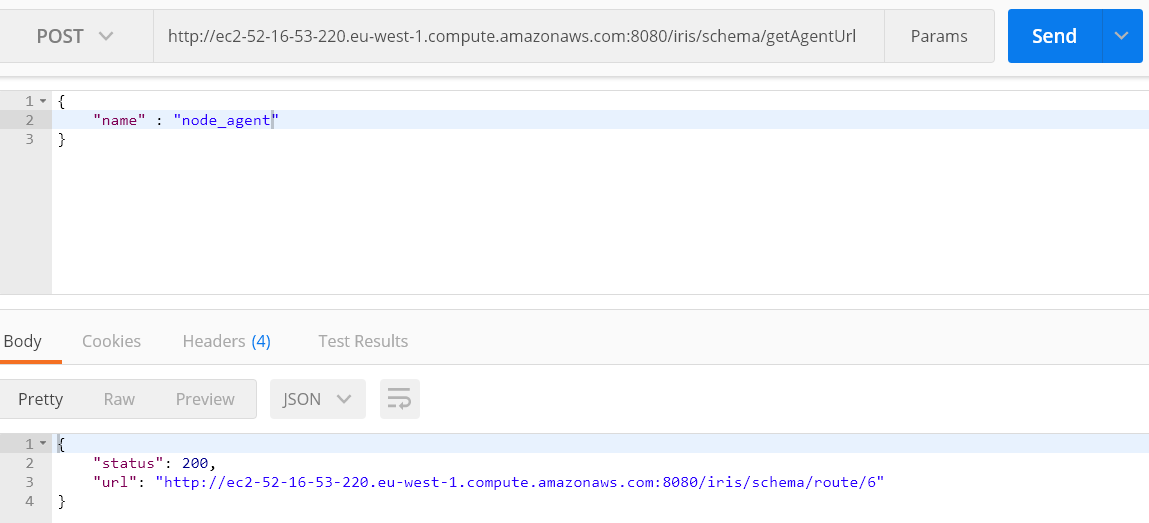
\includegraphics[width=\textwidth,height=\textheight,keepaspectratio]{iris-get-agent-url}
\end{center}
A screenshot of the `getAgentUrl' endpoint being used in Postman to retrieve the Node.js agent's endpoint.
\end{tcolorbox}
\caption{SchemaController `getAgentUrl' endpoint in Postman.}
\end{figure}

\paragraph{Timestamping Data}
Iris now puts a timestamp on all incoming data before it is inserted into Elasticsearch. The timestamp is added as a schema field called `insertionDate' under the schema to which the data belongs. This field is used in the background of the aggregation builder in Iris and will be discussed in that section.

\subsection{Dashboards}

During the Autumn Semester the javascript libraries for building the Iris dashboard system were selected and tested in detail. As a result, the design for implementing the dashboard and updating the charts in realtime has remained essentially  unchanged during the implementation this Semester. The dashboard system features and implementation is discussed in terms of frontend and backend logic in the following sections. A brief overview of how the data flows into the dashboard is also be discussed.
 
\subsubsection{Frontend}
This section will discuss the major factors of the frontend of the Iris dashboard system.

The frontend of the Iris system, is concerned with the charting and dashboard configuration components, which have been built using libraries discussed in the Semester 1 report.

\paragraph{Gridstack.js}

Gridstack.js is a jQuery plugin that provides a drag-and-drop multi-column grid for generic widgets. 
Its features and the basis for selecting gridstack.js is covered in the Semester 1 report.  
 
Due to the extensive research and testing on this library in Semester 1 and the active github support from Gridstack.js developers there was no major issues during the implementation phase in Semester 2. Gridstack.js is used to contain the components (charts) of the dashboard in a grid format. Whenever a chart is created for a dashboard a new container widget is created containing the chart and added to the gridstack grid. This widget automatically becomes resizable, draggable and serialisable.

The logic used to format the gridstack grid into a serialisable object was retrieved from the Gridstack.js serialise demo\footnote{\url{https://dsmorse.github.io/gridster.js/demos/serialize.html}}. Using the basic structure supplied by the gridstack.js developers, the Iris client code was developed and expanded the existing functionality to support chart types and aggregation objects. (see \Cref{fig:Serialization_logic})
%to be included in the serialized data.
\begin{figure}[H]
\centering
\begin{tcolorbox}
    \begin{subfigure}{\textwidth}
        \begin{tcolorbox}
        \centering
        \begin{minted}[breaklines,frame=lines]{javascript}
        this.serializedData = _.map($('.grid-stack > .grid-stack-item:visible'), function (el) {
            el = $(el);
            var node = el.data('_gridstack_node');
            return {
                x: node.x,
                y: node.y,
                width: node.width,
                height: node.height
            };
        }, this);
        \end{minted}
        \caption{Gridstack.js developer's serialization logic.}\label{fig:Serialization_logic}
    \end{tcolorbox}
    \end{subfigure}%
    \newline
    \begin{subfigure}{\textwidth}
        \begin{tcolorbox}
        \centering
        \begin{minted}[breaklines,frame=lines]{javascript}
        serializedData = _.map($('.grid-stack > .grid-stack-item:visible'), function (el) {
        el = $(el);
        var node = el.data('_gridstack_node');
        var widgetInfo = el.data();
        return {
            x: node.x,
            y: node.y,
            width: node.width,
            height: node.height,
            id: node.el[0].id,
            schemaId: widgetInfo.schemaid,
            chartName: widgetInfo.chartname,
            chartType: widgetInfo.charttype,
            data: JSON.parse(localStorage.getItem(node.el[0].id))
        };
    }, this);
        \end{minted}
        \caption{Iris dashboard serialization logic.}
    \end{tcolorbox}
    \end{subfigure}

\end{tcolorbox}
\caption{Iris extension of Gridstack.js serialization}
\end{figure}

One issue with gridstack.js, that was found during the implementation phase, is that the width of a widget can be incorrectly calculated at the upon loading a dashboard. Unfortunately this issue is not consistent and has proven difficult to resolve. Currently the only fix is for the user to click on the resizable handles of a widget and the chart then scales correctly.

For a basic demo of Gridstack.js refer to this url \url{http://gridstackjs.com/demo/}

\paragraph{Billboard.js}

Billboard.js is a charting library based on D3.js. Billboard.js was researched and tested in detail during Semester 1 but was not integrated within Iris until Semester 2.

Integrating Billboard.js into Iris, and more specifically with Gridstack.js, was relatively straight forward, the only issue was sizing issue for loading charts mentioned above.  
Dynamically adding a Billboard.js chart to an existing Gridstack.js grid required an extra parent container to be wrapped around the chart element, effectively converting it to a Gridstack.js widget.

The chart type support will be discussed in \cref{para:charts:fontend} and the chart subscriptions will be discussed in \cref{para:charts:subs:frontend}.

For examples of charts created with Billboard.js see this url \url{https://naver.github.io/billboard.js/demo/}

\paragraph{Chart Types}

\label{para:charts:fontend}
% discuss all the chart types supported
Iris supports the following chart types:
\begin{itemize}
    \item Bar Chart
    \item Bubble Chart
    \item Pie Chart
    \item Line Chart
    \item State Disc Chart (A chart used for monitoring state based data)
    %TODO ADD PIC OF EACH CHART
\end{itemize}

\paragraph{Chart Subscriptions}\label{para:charts:subs:frontend}

The design for how Iris handles sending incoming data to the correct charts is documented in the Semester 1 report. However the design was not implemented until Semester 2. The libraries chosen in Semester 1 for web socket functionality remained the same. Iris uses the Grails Web Socket plugin to add socket communication between dashboard charts and the server, allowing charts to subscribe to incoming data. 

Each client chart on an Iris dashboard subscribes to messages from the server on a unique socket endpoint, which ensures the correct data gets sent to the correct chart. This design is discussed in the Semester 1 report and has remained the same during the implementation of the chart subscription logic in Iris.

For more information on he Grails 3 `grails-spring-websocket' plugin refer to \url{https://github.com/zyro23/grails-spring-websocket}.
\begin{figure}[H]
\begin{tcolorbox}
\begin{minted}[breaklines]{javascript}
function setChartSubscription(subscriptionId, chart, chartType, schemaId){
    //this subscription is for updates being sent to the chart
    client.subscribe("/topic/" + schemaId + "/" + chartType + "/" + subscriptionId, function(message) {
        var parsedMsg = JSON.parse(message.body);
        //update the chart
        if(chartType != chartTypes.StateDisc){  //REGULAR CHARTS
            updateBasicCharts(chart, parsedMsg);
        }else{  //STATE BASED CHARTS
            updateStateDiscChart(chart, parsedMsg);
        }
    });

    //this subscription is for initial loading data for the chart
    client.subscribe("/topic/load/" + schemaId + "/" + chartType + "/" + subscriptionId, function(message){
        var parsedMsg = JSON.parse(message.body);
    // update the chart
        chart.instance.load({
            columns: parsedMsg.data.columns,
            length: 0
        });
    });
}
\end{minted}
\end{tcolorbox}
\caption{Iris client side chart subscription logic.}
\end{figure}

\paragraph{Downloadable Chart Data}

Iris supports the ability to download a JSON file consisting of the current data being displayed on any chart. This functionality was built by using the Billboard.js API and retrieving the chart data, and adding custom logic to format that data into a file to be downloaded upon request.
\begin{figure}[H]
\begin{tcolorbox}
\begin{center}
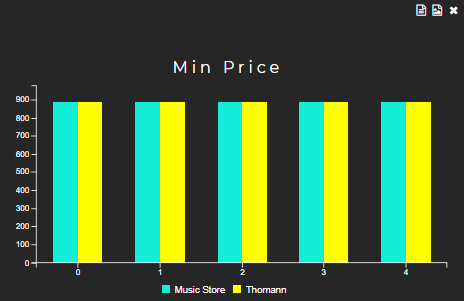
\includegraphics[width=\textwidth,height=\textheight,keepaspectratio]{iris-downloaded-chart}
\end{center}
A screenshot of a downloadable chart in Iris, taken from the `selenium agent' dashboard in Iris. The file icon in the top right is clicked to start the download.
\end{tcolorbox}
\caption{Downloadable chart example.}
\label{fig:downloaded:chart}
\end{figure}

\begin{figure}[H]
\begin{tcolorbox}
\begin{minted}[breaklines]{json}
[{"id":"Music Store","id_org":"Music Store","values":[{"x":0,"value":888,"id":"Music Store","index":0},{"x":1,"value":888,"id":"Music Store","index":1,"name":"Music Store"},{"x":2,"value":888,"id":"Music Store","index":2},{"x":3,"value":888,"id":"Music Store","index":3},{"x":4,"value":888,"id":"Music Store","index":4}]},{"id":"Thomann","id_org":"Thomann",
"values":[{"x":0,"value":888,"id":"Thomann","index":0},
{"x":1,"value":888,"id":"Thomann","index":1,"name":"Thomann"},
{"x":2,"value":888,"id":"Thomann","index":2},
{"x":3,"value":888,"id":"Thomann","index":3},
{"x":4,"value":888,"id":"Thomann","index":4}]}]
\end{minted}
JSON file data downloaded from a chart on the  `selenium agent' dashboard.(Shown in \Cref{fig:downloaded:chart})
\end{tcolorbox}
\caption{JSON file data downloaded from a chart.}
\end{figure}

\paragraph{Revision History}

Iris now supports revision history for all dashboards, meaning a user can navigate between previous versions of a dashboard by simply using a select box on the dashboard page which allows the user select the revision they wish to view. Each revision commit allows a user to write a comment about what changed for the new revision. A user may also delete revisions they no longer wish to keep, once all revisions are deleted then a dashboard is deleted.
\begin{figure}[H]
\begin{tcolorbox}
\begin{center}
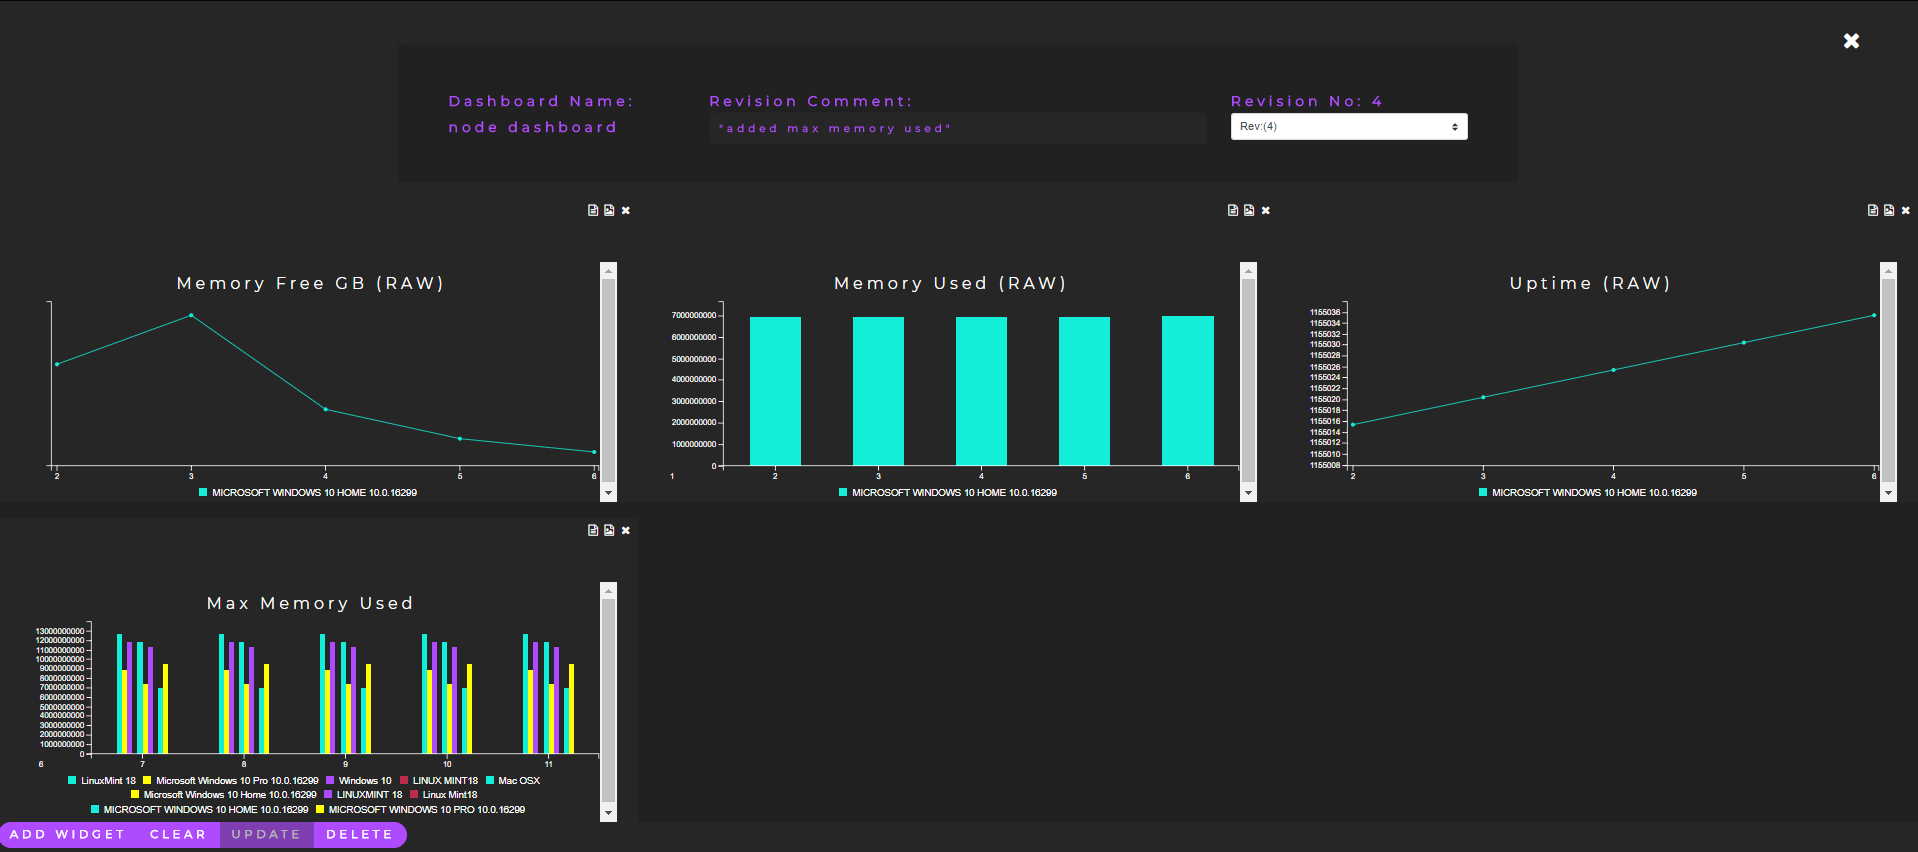
\includegraphics[width=\textwidth,height=\textheight,keepaspectratio]{iris-node-dash-rev-1}
\end{center}
A screenshot of the Node.js dashboard in Iris capturing its fourth revision.
\end{tcolorbox}
\caption{Node.js dashboard revision No. 4.}
\label{fig:dash:rev:4}
\end{figure}
\begin{figure}[H]
\begin{tcolorbox}
\begin{center}
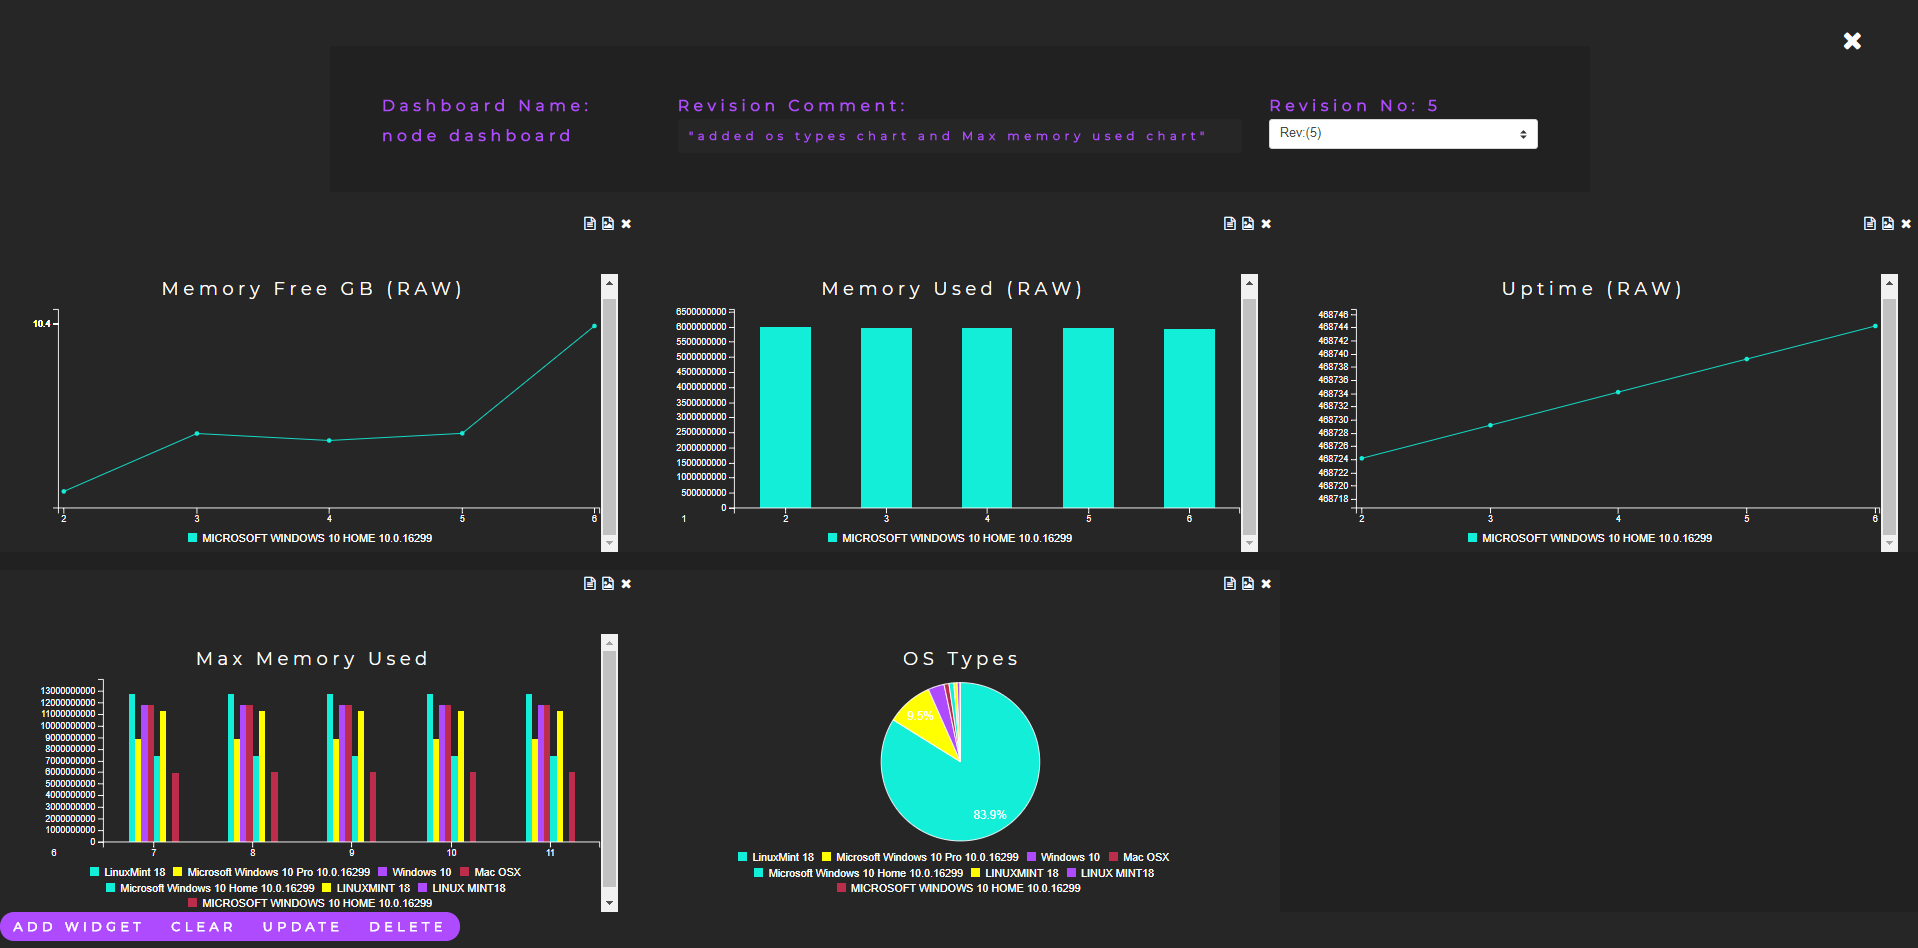
\includegraphics[width=\textwidth,height=\textheight,keepaspectratio]{iris-node-agent-dashboard}
\end{center}
A screenshot of the Node.js dashboard in Iris capturing its fifth revision. Note the extra chart `OS Types' that was added to this revision compared to the fourth revision show in \cref{fig:dash:rev:4}.
\end{tcolorbox}
\caption{Node.js dashboard revision No. 5.}
\end{figure}

\subsubsection{Backend}
This section will focus on the major factors behind the backend implementation of the Iris dashboard system.

Within this section designs from the Semester 1 report will be discussed in terms of their implementation phase during Semester 2 as well as some new features that were designed and added within Semester 2.
\paragraph{Chart Types}
The Iris chart types are handled by using enums in Iris. This allows for the code in Iris to be easily expanded upon when a new chart type is needed, and the use of enums allows for more readable code when dealing with different types of charts.

\begin{figure}[H]
\begin{tcolorbox}
\begin{minted}[breaklines]{groovy}
enum ChartType {

    BAR("Bar"),
    BUBBLE("Bubble"),
    PIE("Pie"),
    LINE("Line"),
    STATE_LIST("StateList"),
    STATE_DISC("StateDisc");

    private String value;

    private ChartType(String value){
        this.value = value;
    }

    String getValue(){ return this.value; }
}
\end{minted}
\end{tcolorbox}
\caption{ChartType.groovy enum from Iris.}
\end{figure}
Due to Iris supporting multiple chart types as well as different types of data, each chart has optional attributes. Some of these optional attributes consist of an Elasticsearch aggregation if the user created the chart using the aggregation builder, and a raw attribute in the case of a user wishing to just send raw data to a chart and not have Elasticsearch perform any aggregations over the incoming data.
\begin{figure}[H]
\begin{tcolorbox}
\begin{minted}[breaklines]{groovy}
class Chart {

    String name
    String chartType
    String subscriptionId
    Aggregation aggregation
    IrisSchema schema
    boolean isRaw = false
    boolean archived = false

    static constraints = {
        name(nullable: false, blank: false)
        chartType(nullable: false, inList: ChartType.values()*.getValue())
        aggregation(nullable: false)
        schema(nullable: false)
        archived(nullable: true)
        subscriptionId(nullable: true)
        isRaw(nullable: true)
    }

    static belongsTo = [grid: Grid]
}
\end{minted}
\end{tcolorbox}
\caption{Chart.groovy domain for representing Charts in Iris.}
\end{figure}

\paragraph{Chart Subscriptions}
When data enters Iris, Iris uses the chart type to figure out how a chart should be updated. For all charts the flow of data is the same, a data source will send data to Iris and Iris will send the data to the chart using a Grails Service which which comes as part of the `grails-spring-websocket' plugin. If a chart is marked as raw or of type `State Disc' then the data being sent to the chart is not modified, if a chart instance has an Elasticsearch aggregation attached to it the aggregation is executed in Elasticsearch and the result is parsed and formatted to suit the chart type and then sent to the chart to be updated on the frontend.

\paragraph{Serilization}
Iris serializes Dashboard domains through composition. Each Dashboard domain has a Grid domain object which stores the entire dashboard in JSON. This means that serializing and loading dashboards is simply done with a string of JSON. This JSON is passed to the frontend where it is parsed by the client to create the dashboard.

Due to Iris storing the dashboard grid as a JSON string, it allows for Iris to extend its dashboard system in the future by allowing users to build dashboards offline or locally and upload a JSON file which represents their dashboard. Iris will be able to save and load the dashboard as long as the user conforms to the existing dashboard JSON structure which is in place.

\paragraph{Revision History}
Iris supports revision history for its dashboard system. When a dashboard is initially created Iris will create a new Revision domain object to associate with the dashboard. This revision object has a unique id which is referred to as the `revisionId', this id is specific to each dashboard. Along with the revision id, a revision number is also stored, meaning all revisions specific to a dashboard have the same revision id and different revision numbers. Whenever a dashboard is updated and the changes are committed, Iris will create a new revision for the dashboard by coping the revision id of the most recent revision and then incrementing the revision number of the most recent revision. This results in a brand new revision being created. When a dashboard is rendered on the frontend of Iris the backend sends down all the revisions associated with the dashboard which allows the user to select what version of the dashboard they wish to view.

\begin{figure}[H]
\begin{tcolorbox}
\begin{center}
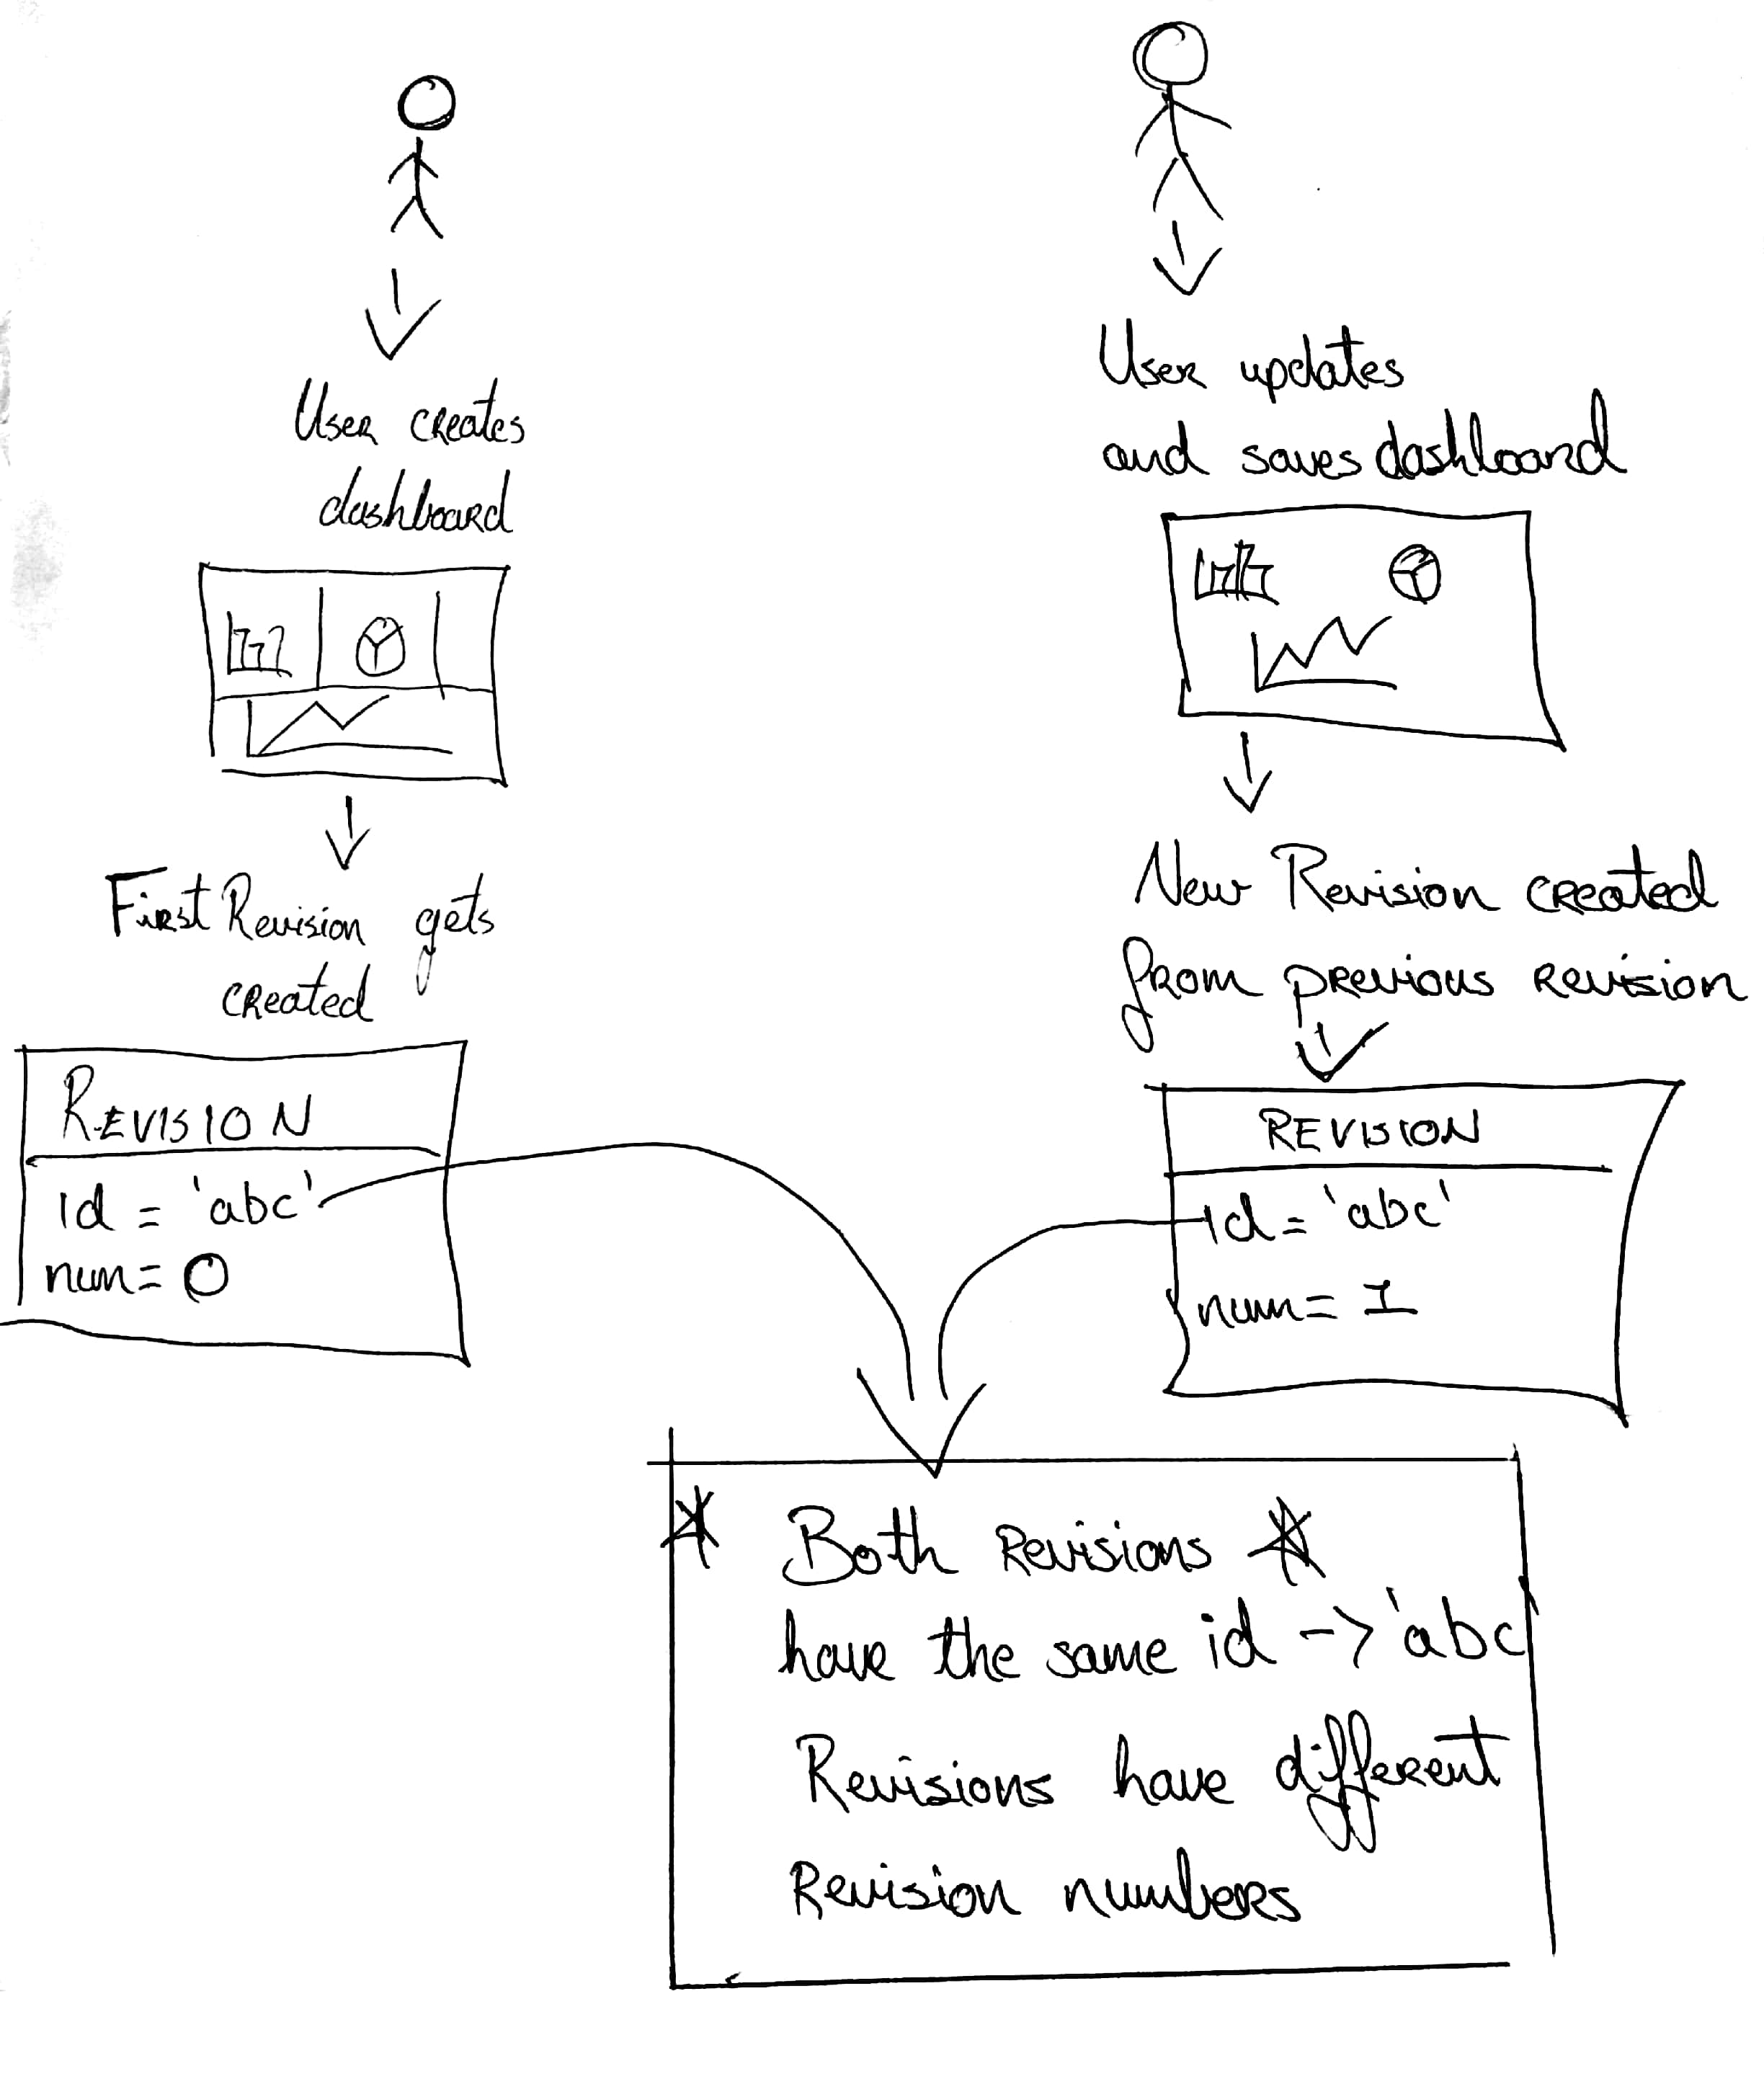
\includegraphics[width=\textwidth,height=\textheight,keepaspectratio]{iris-dash-revision}
\end{center}
An image showing how the revision history of dashboards works in Iris.
\end{tcolorbox}
\caption{Iris dashboard revision diagram.}
\end{figure}

\paragraph{Scalability}
A big concern with Iris in the beginning was to see how scalable the dashboard system would be if a lot of data was being sent to Iris. In an effort to make the dashboard system more efficient Iris dashboards have a boolean attribute called `isRendering'. When a dashboard is being viewed by a user the backend toggles the `isRendering' state of the dashboard to true, this is switched to false once a dashboard is no longer being viewed. The reason for this is to prevent data being modified and formatted for a dashboard which is not being rendered to the user. By having this state attached to a dashboard, a dashboard will only be sent updates if it is being viewed by a user, otherwise the data will simply be entered into Elasticsearch and no more code will be executed. This makes the dashboards much more efficient and scalable as Iris is only dealing with dashboards that are being viewed.


%QUESTION - how is this implemented? Is it a heartbeat ?

%ANSWER - no it's not as good as a heartbeat unfortunately. When a dashboard is opened an ajax call is made to the server to toggle the state of the specific dashboard. On the client side the dashboard is saved in local storage, once a user closes the dashboard the dashboard home page is loaded, upon load it checks to see if there are any rendering dashboards in local storage, if so ajax calls are made to toggle there state again and mark them as not rendering on the server. A heartbeat would be a better way of doing things, the websockets work using a heartbeat. Another idea I had was similar to my first approach but to cache the dashboards on the server side with no 'isRendering' attribute, as any dashboard in that cache would be considered to be rendering, this would save me some database calls and would probably be more efficient. However I am too lazy to go change things now.

\begin{figure}[H]
\begin{tcolorbox}
\begin{center}
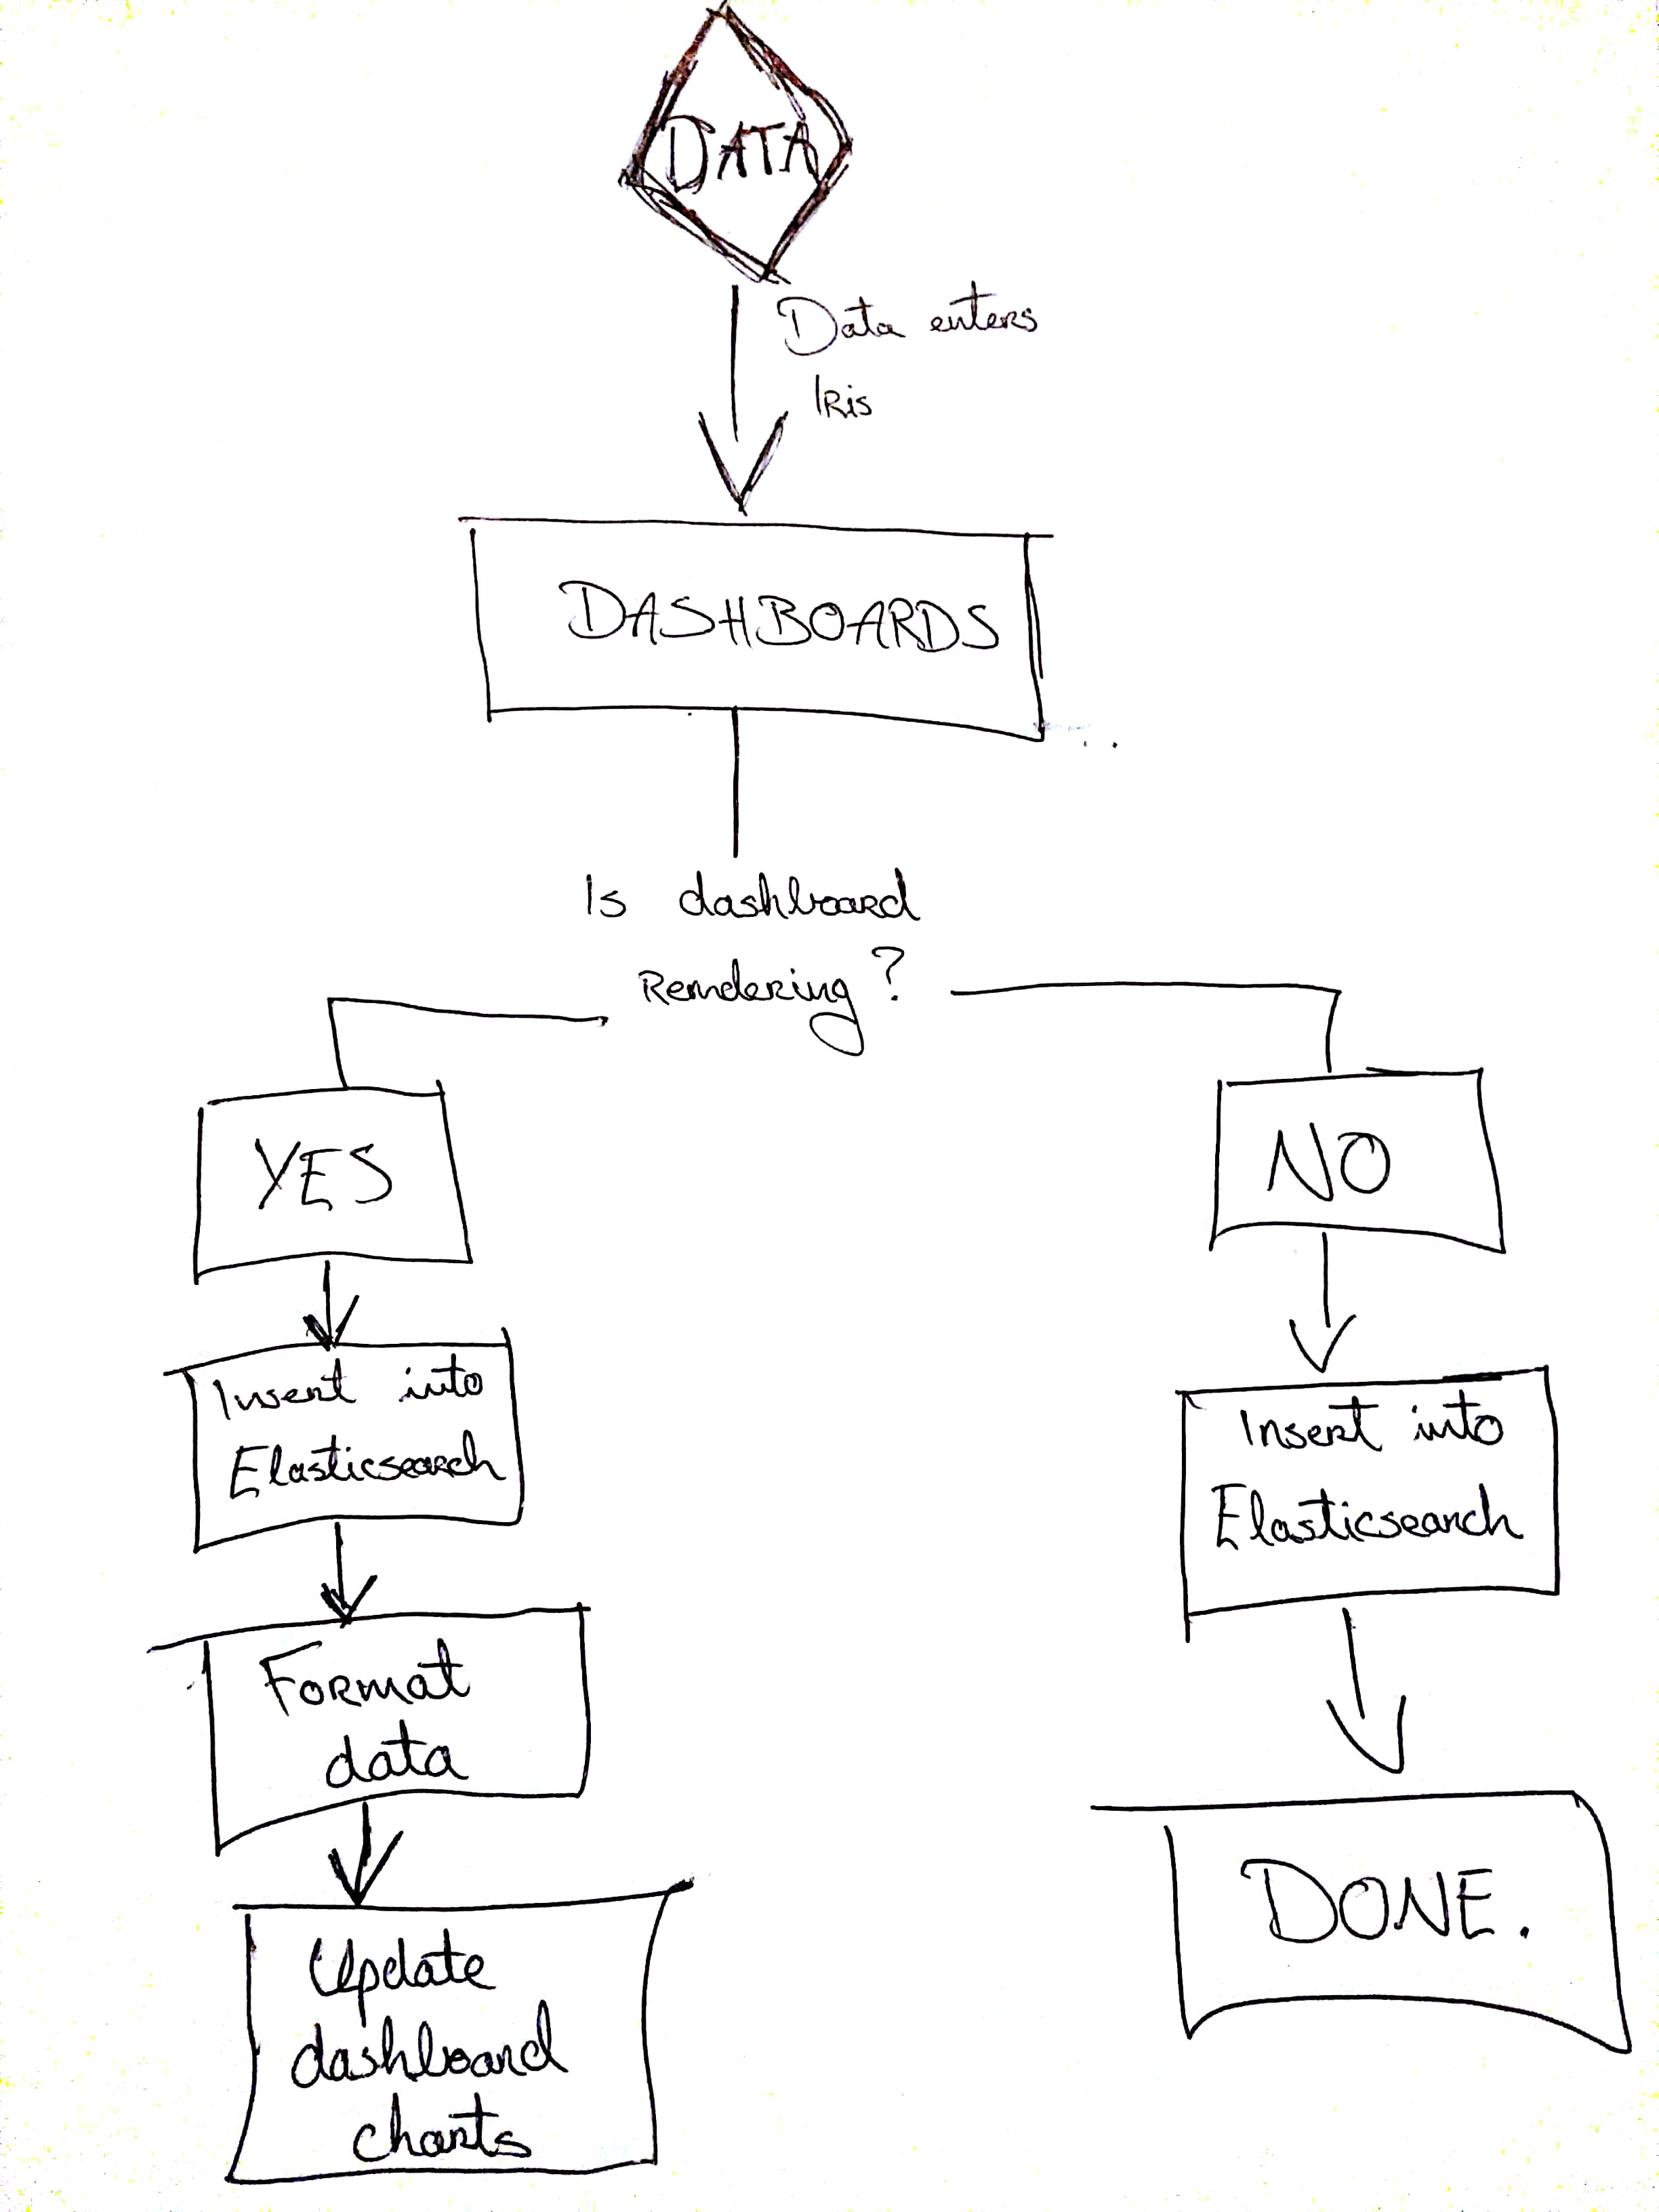
\includegraphics[width=\textwidth,height=\textheight,keepaspectratio]{iris-dash-scalability}
\end{center}
A flow chart showing how Iris handles dashboards that are rendering versus dashboards that are not rendering.
\end{tcolorbox}
\caption{Iris dashboard scalability.}
\end{figure}

\paragraph{User Specific}
In the Semester 1 report similar dashboard tools were compared with the design for Iris. One of the most obvious tools to compare against Iris was Kibana due to it being apart of the ELK (Elasticsearch, Logstash, Kibana) stack. In the Semester 1 report it was discussed that Kibana does not support user specific dashboards, meaning all users can see all dashboards. Iris treats both dashboards and schemas as being user specific, meaning each user has their own personal set of dashboards in comparison to Kibana which does not.

\subsection{Aggregation Builder}
The aggregation builder was partially implemented in Semester 1, the aggregation types were in place and the logic for building an Elasticsearch aggregation through the Iris UI were in place. In Semester 2 some more features were added to allow for more fine grained data monitoring. In the following sections the current aggregation types that Iris supports are listed and the new aggregation builder previewer are discussed.

\subsubsection{Aggregation Types}

% List all possible aggregations you can test
In this section the aggregations which Iris currently supports are discussed. The following list contains the aggregations that Iris can currently build through the aggregation builder.
\begin{itemize}
    \item Average (Calculates the average of a numerical field).
    \item Cardinality (Calculates the approximate count of distinct values).
    \item Stats (Returns basic stats on a numerical field such as count, min, max, avg, sum).
    \item Extended Stats (Returns a grouping of stats on a numerical field such as max, min, count, avg, sum, sum of squares, variance, standard deviation).
    \item Max (Calculates the max of a numerical field).
    \item Min (Calculates the min of a numerical field).
    \item Sum (Calculates the sum of a numerical field).
    \item Value Count (Calculates the number of values extracted from aggregated documents).
\end{itemize}  
Some of the aggregations listed above are not suited for use on charts as the data they return are not suited for charts, for example the stats and extended stats aggregations would not be ideal for fitting to a chart. However they are very useful to get an overall view of the data quickly without having to worry about fitting the data to a chart.
\begin{figure}[H]
\begin{tcolorbox}
\begin{center}

\includegraphics[width=\textwidth,height=\textheight,keepaspectratio]{iris-agg-options}
\end{center}
A screenshot showing the aggregation options available inside the Iris aggregation builder.
\end{tcolorbox}
\caption{Iris aggregation builder options.}
\end{figure}

In Semester 1 the aggregations were running over all documents in the Elasticsearch index, this was fine for demonstrating the aggregation builder's ability to build aggregations, but for realtime data this would be an expensive way to run aggregations, especially if the Elasticsearch index contained a large amount of data. To tackle this issue there was an option to run aggregations over the most recent entries in the Elasticsearch index and to specify how many entries you want to run the aggregation over. This is a powerful modification to the aggregation builder as now users can take advantage of creating charts that display moving averages, minimums and maximums, as well as avoid running an aggregation over all of the entries in the Elasticsearch index which would be slow. 
\begin{figure}[H]
\begin{tcolorbox}
\begin{center}
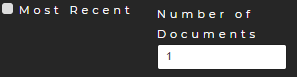
\includegraphics[width=\textwidth,height=\textheight,keepaspectratio]{iris-agg-recent}
\end{center}
A screenshot showing the aggregation most recent option.
\end{tcolorbox}
\caption{Iris aggregation most recent option.}
\end{figure}

It is not advisable to create aggregations for charts which are not run over the most recent entries, especially if the data in the Elasticsearch index is large. If a user wishes to run these aggregations they should do so in the aggregation builder area, where no dashboards need to be updated and time is not a concern.

\subsubsection{Aggregation Builder Preview}
Iris now supports a preview of the aggregation JSON object being built as the user interacts with the aggregation builder UI. This gives the user a look into how the aggregation objects are constructed and allows them to copy the aggregation object in case they wish to execute the aggregation outside of Iris and don't know how to construct an Elasticsearch aggregation.
\begin{figure}[H]
\begin{tcolorbox}
\begin{center}
\begin{subfigure}{0.5\textwidth}
\centering
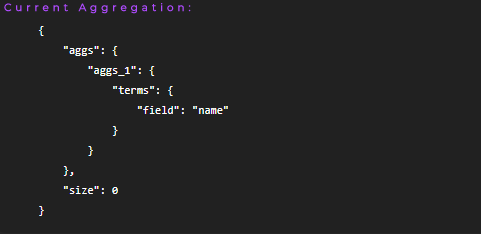
\includegraphics[width=0.9\linewidth]{iris-current-agg-1}
\caption{Current aggregation with one level.}
\end{subfigure}%
\begin{subfigure}{0.5\textwidth}
\centering
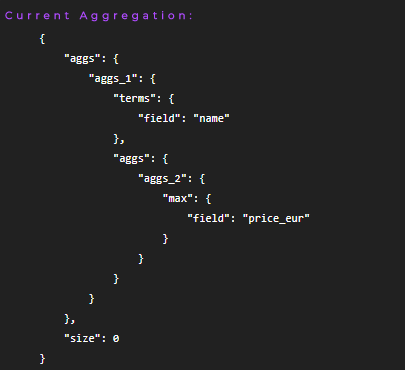
\includegraphics[width=\linewidth]{iris-current-agg-2}
\caption{Current aggregation after nesting an aggregation inside the previous aggregation.}
\end{subfigure}
\end{center}
\end{tcolorbox}
\caption{Iris aggregation builder preview.}
\end{figure}

\subsubsection{Testing Aggregations}
In Semester 1 it was demonstrated that Iris test users could use the aggregation builder area to test their aggregations before putting using the aggregation for a chart. However the aggregation builder was on a different page to that of the dashboards. In Semester 2 the aggregation builder was added to the dashboard creation area, giving users the full functionality of the aggregation builder as they make a chart for a dashboard. This allows a user to test their aggregations before saving a chart to a dashboard to make sure the data being returned is satisfactory.

\begin{figure}[H]
\begin{tcolorbox}
\begin{center}
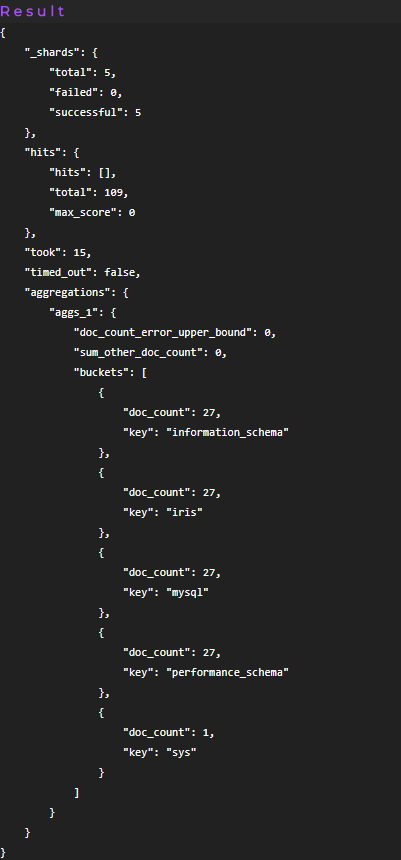
\includegraphics[width=0.8\textwidth,height=0.8\textheight]{iris-agg-test}
\end{center}
A screenshot showing the aggregation result returned from testing an aggregation inside the aggregation builder area.
\end{tcolorbox}
\caption{Iris aggregation test result (aggregation builder area).}
\end{figure}

\begin{figure}[H]
\begin{tcolorbox}
\begin{center}
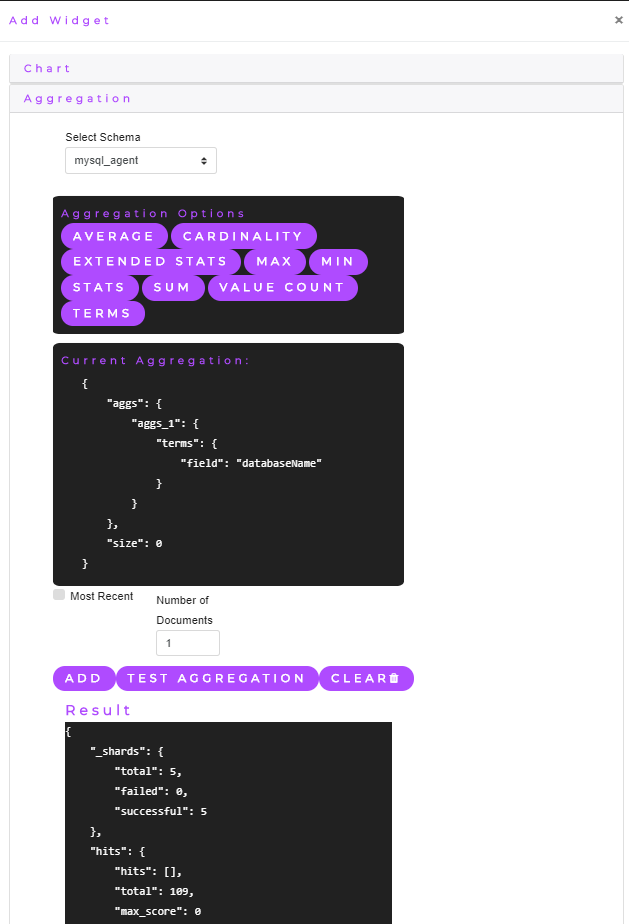
\includegraphics[width=\textwidth,height=\textheight,keepaspectratio]{iris-chart-agg-builder}
\end{center}
A screenshot showing the aggregation builder in the dashboard section.
\end{tcolorbox}
\caption{Iris aggregation test result (Dashboard area).}
\end{figure}
\subsection{Security}
% talk about the addition of security in iris
In Semester 1 it was mentioned that the Grails Spring Security plugin would be used for authentication in Iris. The following sections discusses the security improvements made from Semester 1 to Semester 2.

\subsubsection{Spring Security Core Plugin}
In Semester 1 Iris used the Spring Security Core plugin to create Users, Roles and User Roles. The plugin allowed Iris to authenticate all endpoints by not allowing a user access to the web application unless they are a valid user who has been fully authenticated i.e logged in.

A basic role association was created for the user called `ROLE\_USER'. This tells Iris what access a user with this specific role has within the web application.

Spring Security also automatically deals with hashing passwords for users which adds an extra layer of security for users.
\subsubsection{Spring Security REST Plugin}
Throughout Semester 2 it was apparent that the data sources sending data to Iris needed to be authenticated as they may be posing as a fake data source. The Grails Spring Security Rest plugin was decided upon as being an appropriate way to authenticate data sources accessing Iris API endpoints.

The plugin allows a user to login to Iris using a POST request which contains their credentials in a JSON payload. If a user is successfully authenticated Iris responds with a JWT (JSON Web Token) for the user to send as part of future requests to the Iris API endpoints. If a request is received with a valid JWT token in the X-Auth-Token header the data source is granted access to the API endpoint.


\begin{figure}[H]
\begin{tcolorbox}
\begin{center}
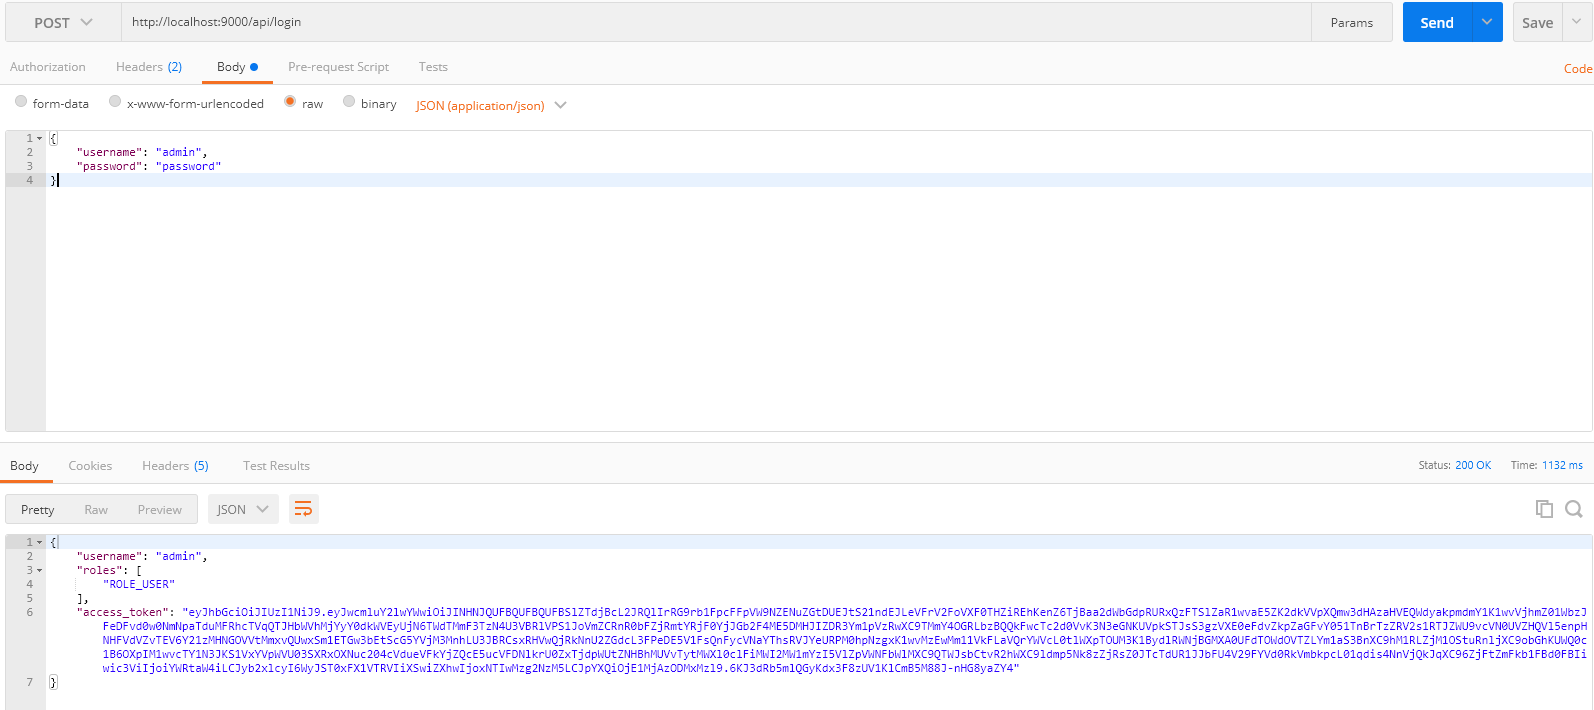
\includegraphics[width=\textwidth,height=\textheight,keepaspectratio]{iris-api-login}
\end{center}
A screenshot showing Iris API login being used to authenticate a valid Iris user, note the JWT token that was sent back.
\end{tcolorbox}
\caption{Iris login API.}
\end{figure}

\begin{figure}[H]
\begin{tcolorbox}
\begin{center}
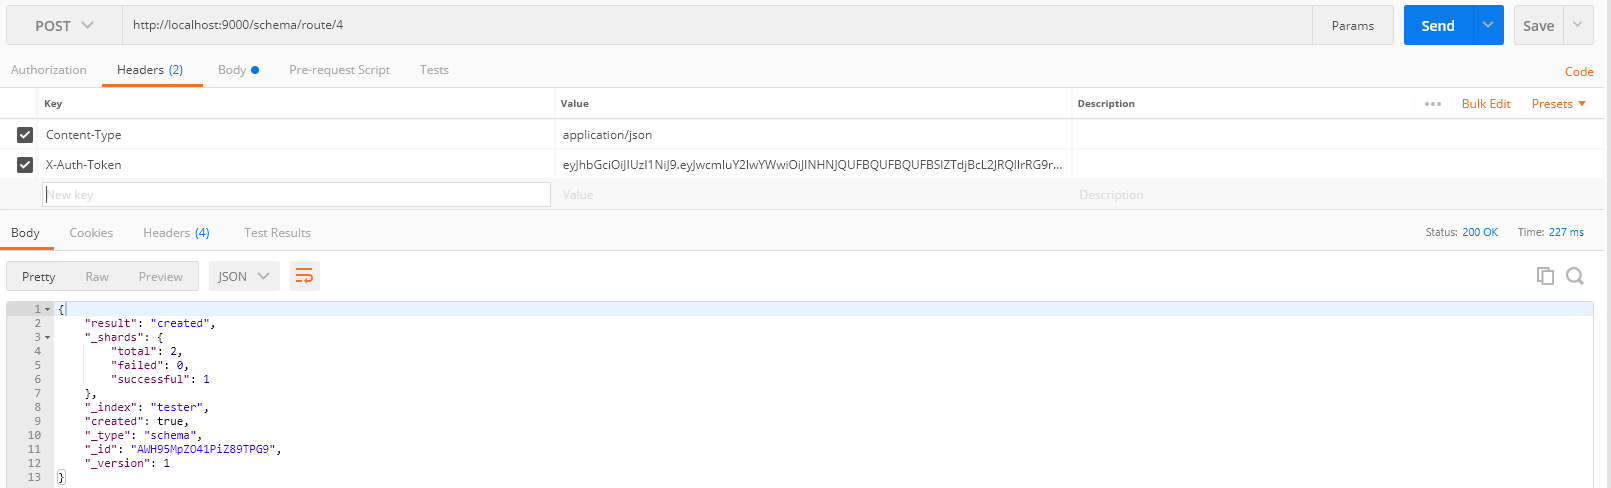
\includegraphics[width=\textwidth,height=\textheight,keepaspectratio]{iris-api-header}
\end{center}
A screenshot showing a data source being authenticated by its JWT in the `X-Auth-Token' header of the request.
\end{tcolorbox}
\caption{Iris JWT validation.}
\end{figure}

If the user's credentials are invalid or the JWT sent by the data source is invalid the user will be denied access to the endpoint.

\begin{figure}[H]
\begin{tcolorbox}
\begin{center}
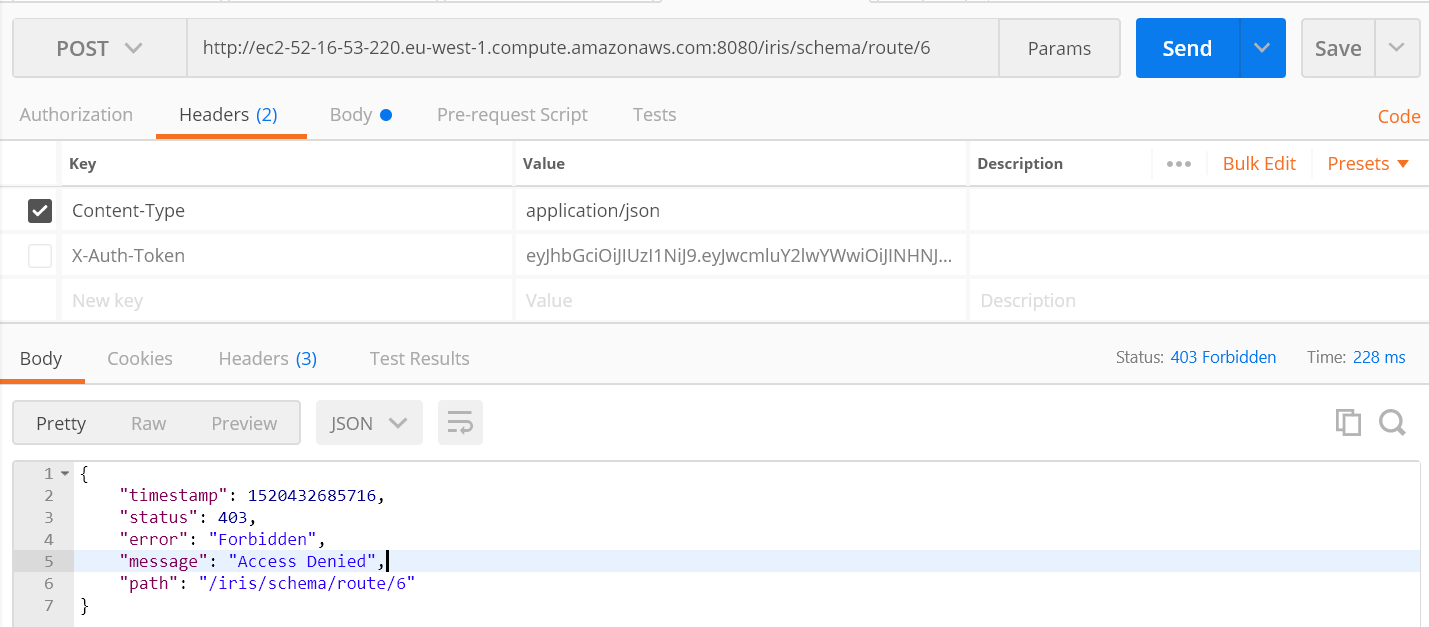
\includegraphics[width=\textwidth,height=\textheight,keepaspectratio]{iris-access-denied}
\end{center}
A screenshot showing the access denied message recieved upon authentication failure with Iris.
\end{tcolorbox}
\caption{Iris API access denied example.}
\end{figure}

Using the plugin, Iris configured its endpoint security based on the endpoints available to the user. All endpoints which are part of the frontend of Iris are locked unless a user is fully authenticated, meaning a user must sign in to use any of the user interface of Iris.

The two REST endpoints Iris exposes to data sources are `/schema/route/' and `/schema/getAgentUrl'. These endpoints are used by data sources to get unique schema endpoints and sent data to Iris. Both of these endpoints are secured and need authentication by logging in using the previously mentioned `/api/login' as well as a valid JWT. In the backend of Iris these methods are also marked as needing a user with the `ROLE\_USER' role to be given access.

\begin{figure}[H]
\begin{tcolorbox}
\begin{center}
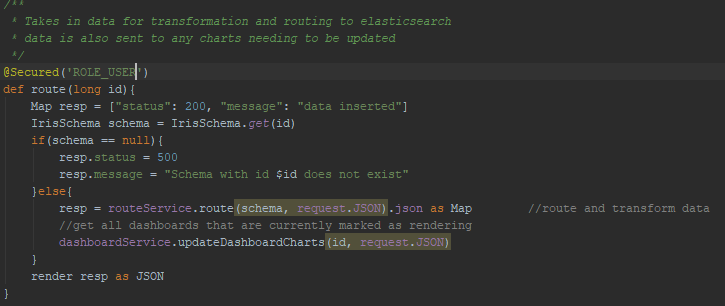
\includegraphics[width=\textwidth,height=\textheight,keepaspectratio]{iris-secured-route}
\end{center}
A screenshot showing the `/schema/route/' endpoint being secured with the `Secured' annotation.
\end{tcolorbox}
\caption{Iris secured route.}
\end{figure}

The only endpoints in Iris that require no authentication are the `/login/auth' endpoint which returns the login page for a user who is using the web application to login and the `/api/login' for a data source who is logging in through a POST request. All other endpoints are secured.

\begin{figure}[H]
\begin{tcolorbox}
\begin{center}
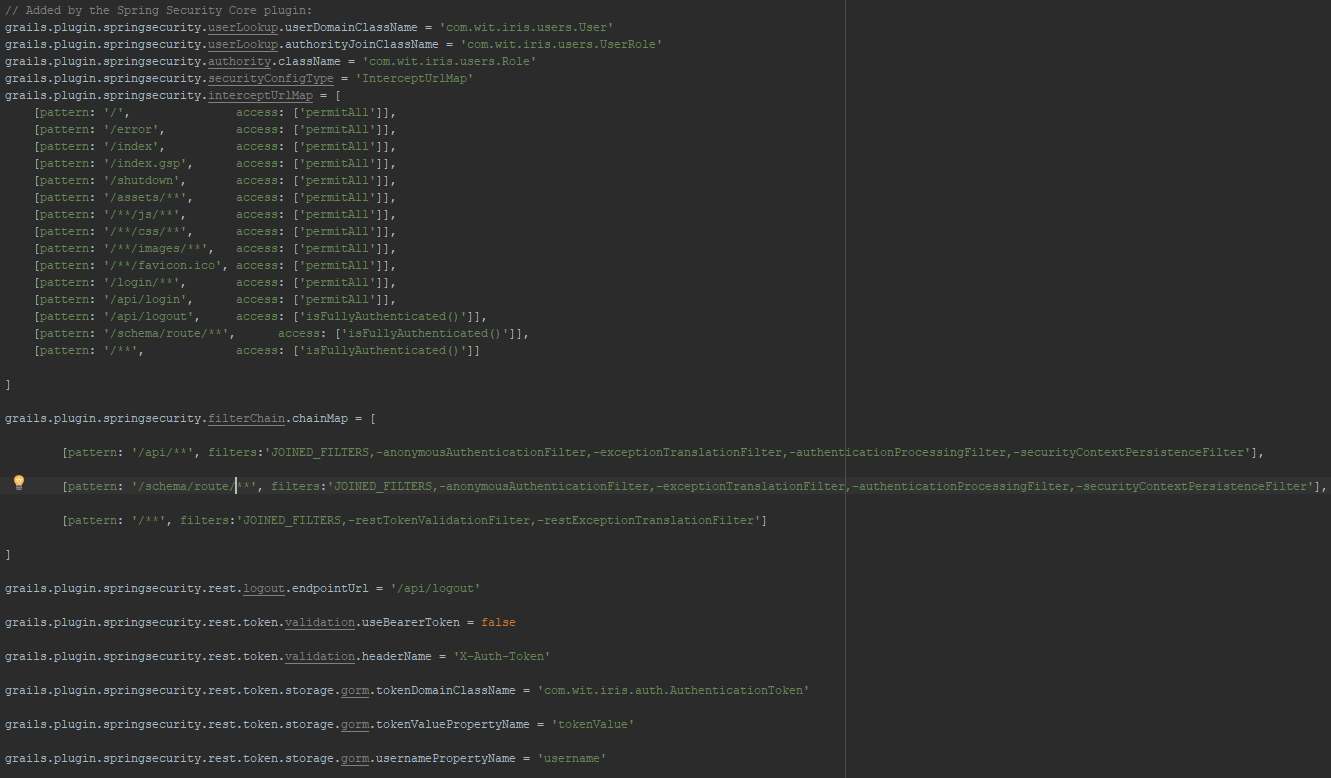
\includegraphics[width=\textwidth,height=\textheight,keepaspectratio]{iris-spring-security-config}
\end{center}
A screenshot showing the spring security configuration settings for all of the Iris endpoints.
\end{tcolorbox}
\caption{Iris spring security configuration file.}
\end{figure}

For more information on JWT, Spring Security Core and Spring Security Rest, please refer to these urls:
\begin{itemize}
    \item JWT - \url{https://jwt.io/}
    \item Spring Security Core - \url{https://github.com/grails-plugins/grails-spring-security-core}
    \item Spring Security Rest - \url{https://github.com/alvarosanchez/grails-spring-security-rest}
\end{itemize}


\subsubsection{Data Source Adaptation}
Data sources communicating with Iris now need to get authenticated by sending valid user credentials to the `/api/login' endpoint. The data source must then use the JWT token with every request as part of the X-Auth-Token header which was given to them from Iris upon successfully logging in.

The data sources used to test Iris have hardcoded JWTs in their code to make testing easier, however all real use cases must use the `/login/api' to retrieve their JWTs.

\section{Data Sources}
A data source can be any process that generates data and pushes it to Iris. In \cref{s:implementation:datasource}
a number of examples of data sources are discussed. The implementation details of these data sources is not covered in detail because they are not germane to the this project and follow well know patterns.

\chapter{Deployment, Testing and Evaluation}
In this chapter the procedure to deploy, test and evaluate Iris is discussed. In the Semester 1 report the deployment was not taken into consideration meaning the deployment section is fundamentally new. The testing and evaluation of data sources is new in regards to the data sources being created and tested against Iris, however they were briefly discussed in the Semester 1 report in regards to what their overall interaction with Iris would be. The details of what data the data sources would send and what platform they would use to send the data were not discussed.
\section{Deployment}
In this section the procedure of deploying Iris will be discussed in terms of how the application is is built and served as well as how it interacts with Elasticsearch and MySQL instances while in production.
\subsection{AWS (Amazon Web Services)}
Amazon Web Services is used to host Iris as well as host the Elasticsearch and MySQL processes which Iris interacts with, these will be discussed in the following subsections.
\subsubsection{EC2 Instance}
\label{sub:ec2}
Iris is hosted on an AWS EC2 instance. The instance is part of the free tier options meaning the instance is limited in regards to its hardware specifications which can be found in \cref{table:ec2:specs}. The EC2 instance is configured to allow incoming HTTP requests on port 8080 so that users can send requests to Iris as well as receive responses from Iris. The EC2 instance also runs the MySQL process where Iris stores its user related data which will be discussed in \cref{sub:mysql:instance}.
\begin{table}[H]
\centering
\small
\setlength\tabcolsep{6pt}
 \begin{tabular}{|c|c|c|c|}
 \hline
 Model & vCPU & Memory & Storage\\
 \hline\hline
 t2.micro & 1 & 1GB & 8GB\\ 
 \hline
\end{tabular}
\caption{AWS EC2 instance specifications.}
\label{table:ec2:specs}
\end{table}

For more information on the EC2 instance types refer to this url \url{https://aws.amazon.com/ec2/instance-types/}.

\subsubsection{Jetty}
Jetty is an open source HTTP server that can be used to act as web application container. Jetty was not the first choice for being the container for Iris. Tomcat was the original choice as Onaware have their java web applications in Tomcat instances, this meant Iris was also going to be a candidate for being put in a Tomcat container. However due to the limitations of the EC2 instance mentioned in \cref{table:ec2:specs}, Tomcat proved to be unstable and was running out of memory for the JVM (Java Virtual Machine) once it was launched. 

Due to Tomcats' instability, a different web application container was required. Several other containers were tested including GlassFish and JBoss, but these containers also failed to deploy Iris due to limited memory. Jetty was then tested and deployed Iris successfully. In order to test the deployment, the Jetty container was launched and shutdown several times over several days to ensure the container was stable. Once Jetty proved to be satisfactory Iris was deployed.

For more information on Jetty refer to this url \url{https://www.eclipse.org/jetty/documentation/9.4.x/introduction.html}.
\subsubsection{Elasticsearch Instance}
The Elasticsearch instance which Iris interacts with is hosted on AWS as part of the Elasticsearch Services offered by Amazon. The instance is part of the free tier selection but proved to have sufficient hardware specifications for Iris which are detailed in \cref{table:elastic:specs}. The instance was tested heavily by sending requests from Iris at a rapid and constant rate over a period of time. The instance did not appear to have any issues dealing with the requests and was considered suitable for Iris.
\begin{table}[H]
\centering
\small
\setlength\tabcolsep{6pt}
 \begin{tabular}{|c|c|c|c|}
 \hline
 E.S Version & Documents & Storage\\
 \hline\hline
 5.5 & 46,590 & 7.22GB\\ 
 \hline
\end{tabular}
\caption{AWS Elasticsearch instance specifications.}
\label{table:elastic:specs}
\end{table}
\subsubsection{MySQL Instance}
\label{sub:mysql:instance}
The MySQL instance that Iris uses to store user specific data such as schemas, dashboards etc.\ is run on the EC2 mentioned in \cref{sub:ec2}. This allowed Iris to configure its database connector to use localhost, which made development and production environments easier to test as the database configuration was the same.
\section{Testing and Evaluation --- Data Sources}
\label{s:implementation:datasource}
A number of data sources have been implemented to demonstrate the flexibility of Iris and to test the aggregation of data from Iris into Elasticsearch. Each of the following sections describe a data source and its unique features.

\subsection{Android App}
\subsubsection{Description}
The android application demonstrates how Iris handles state based data. The application is very simple, but demonstrates how simple it is to monitor an application's state through Iris. The application is simply a screen consisting of six tiles. Each tile represents a different state, each state has three colours and three numerical values linked to the states and colours. The android application allows the user to change the states of these tiles, which then changes the state of the tile colour and value. When a user is satisfied with the states they wish to send to Iris they simply tap the screen. This results in a JSON object being sent to Iris consisting of the current numerical value for each state tile i.e the current state of the tiles.
%Iris Android app screenshot
\begin{figure}[H]
\begin{tcolorbox}
\begin{center}
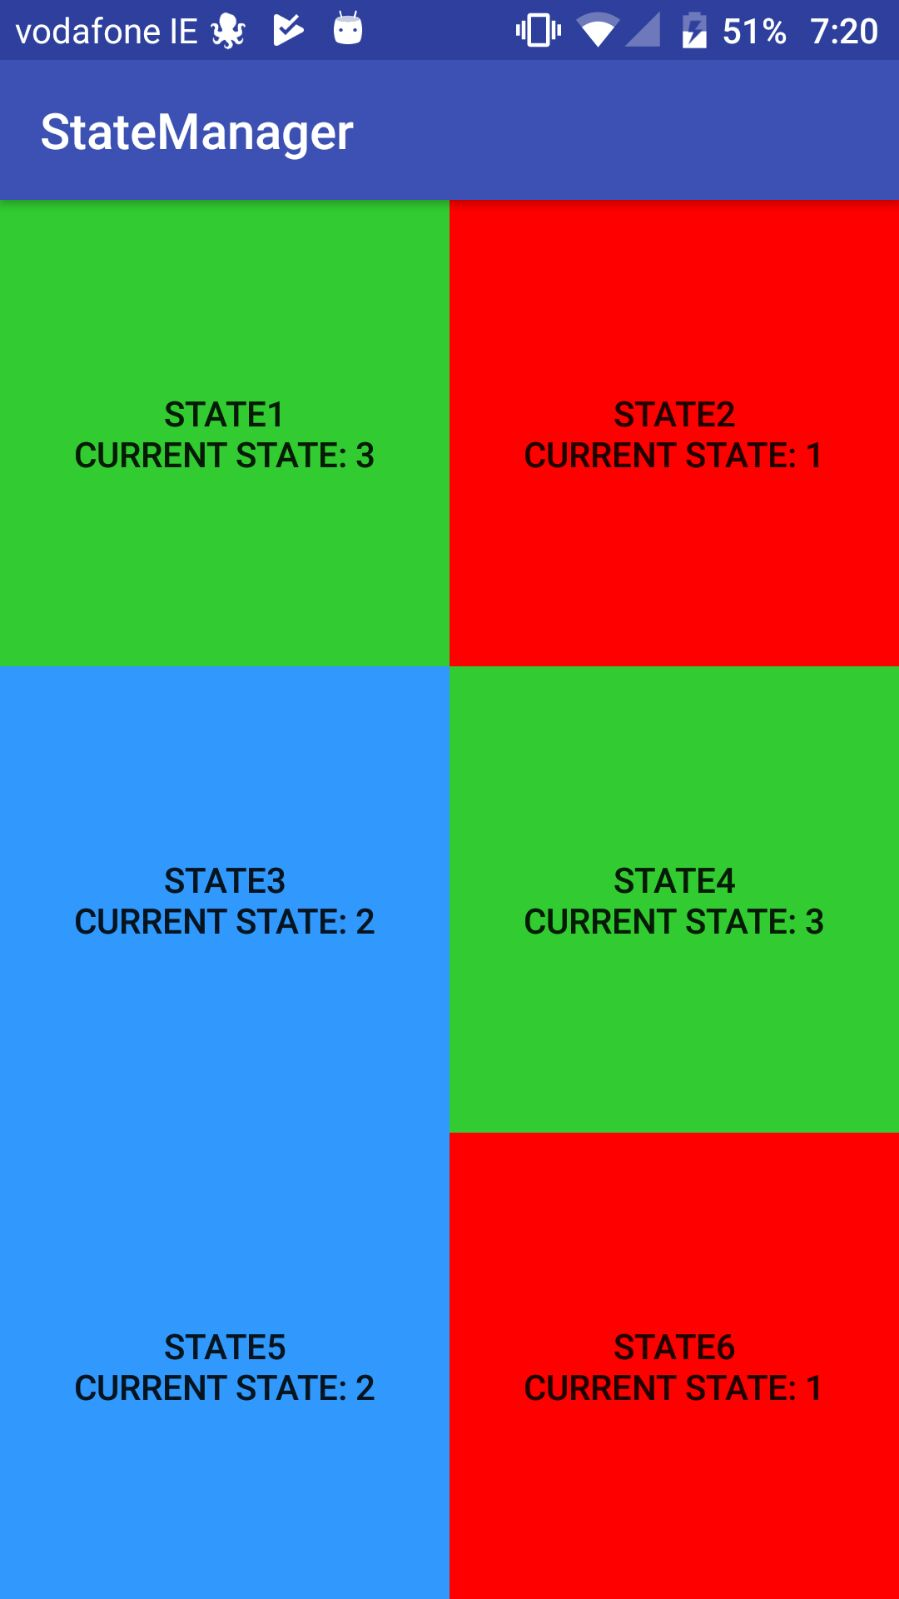
\includegraphics[width=0.7\textwidth,height=0.7\textheight]{android-agent}
\end{center}
A screenshot of the android agent and its state based tiles. Each of the tiles on the screen holds a state, the states are as follows:
\begin{itemize}
    \item State 1 - Values:(1, 2, 3), Colours:(Red, Blue, Green)
    \item State 2 - Values:(1, 2, 3), Colours:(Red, Blue, Green) 
    \item State 3 - Values:(1, 2, 3), Colours:(Red, Blue, Green) 
    \item State 4 - Values:(1, 2, 3), Colours:(Red, Blue, Green) 
    \item State 5 - Values:(1, 2, 3), Colours:(Red, Blue, Green) 
    \item State 6 - Values:(1, 2, 3), Colours:(Red, Blue, Green) 
\end{itemize}
\end{tcolorbox}
\caption{Android agent for Iris.}
\end{figure}

\subsubsection{Linkage with Iris}
The android application is linked to Iris through a unique REST endpoint specific to the android agent schema. All of the data being sent from the android application is sent to this endpoint. Once the data enters Iris, Iris will run through it's logic for checking for dashboards and charts associated with the schema and send the data through to the charts. 
%Add a ref to a section where you explain what iris does, so you dont have to keep repeating this for all agents
In this case the charts are state based and will update according to the state values that are given to them.

\begin{figure}[H]
\begin{tcolorbox}
\begin{center}
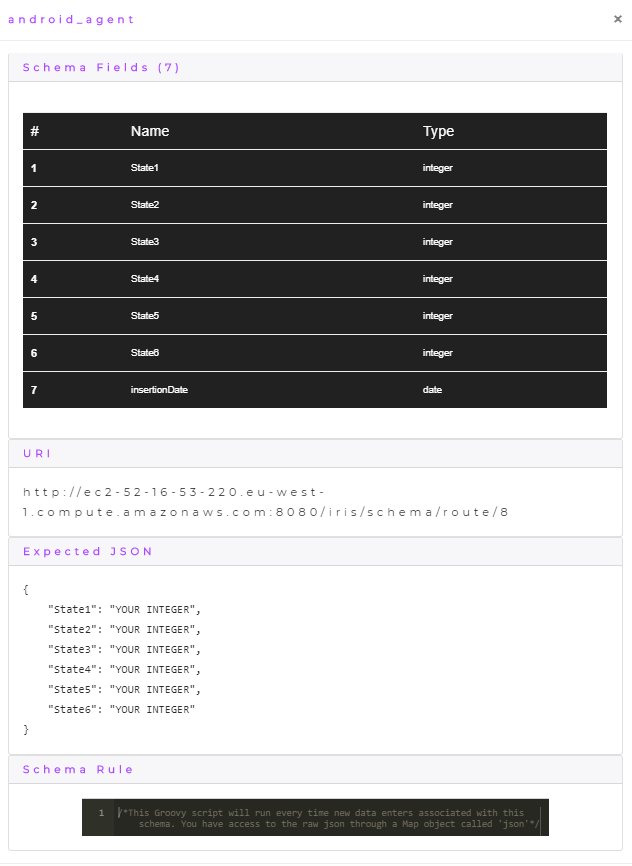
\includegraphics[width=\textwidth,height=\textheight,keepaspectratio]{iris-android-schema}
\end{center}
A screenshot of the Android agent schema in Iris.
\end{tcolorbox}
\caption{Android agent schema in Iris.}
\end{figure}

%Iris Android agent dashboard screenshot
\begin{figure}[H]
\begin{tcolorbox}
\begin{center}
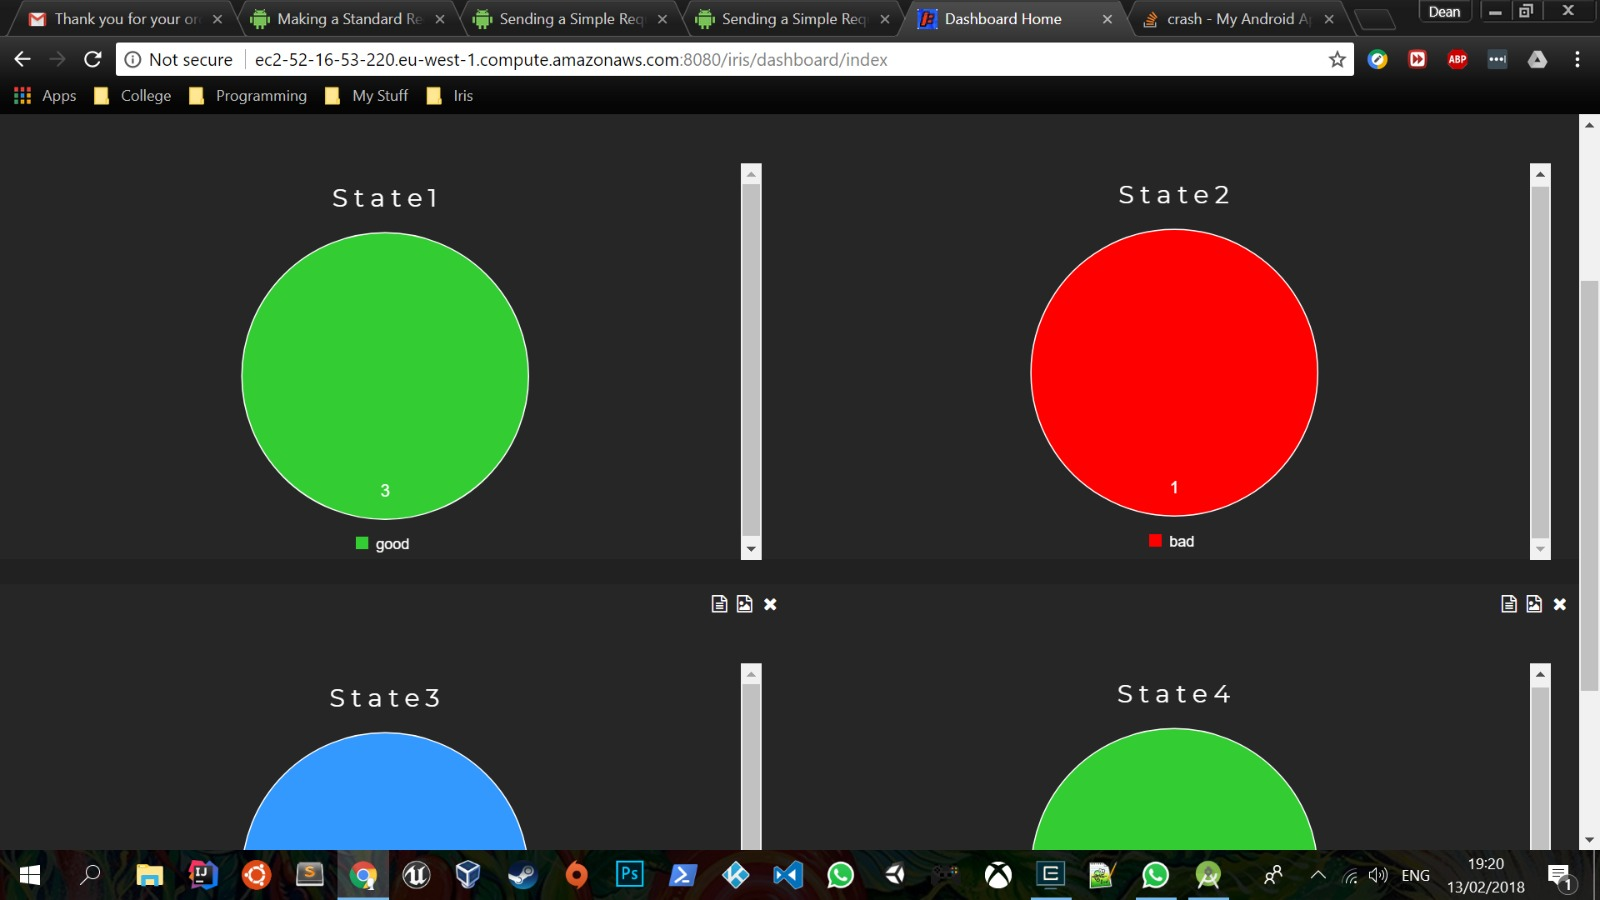
\includegraphics[width=\textwidth,height=\textheight,keepaspectratio]{iris-android-dashboard}
\end{center}
A screenshot of the android agent dashboard in Iris and its state based tiles.
\end{tcolorbox}
\caption{Android agent dashboard in Iris.}
\end{figure}

\subsection{Raspberry Pi}
The Raspberry Pi agent is used to demonstrate the plug and play ability of a Raspberry Pi combined with the versatility of Iris.

\subsubsection{Description}
The Raspberry Pi agent demonstrates how a user can use a Raspberry Pi to run a script to continuously monitor an API. In the case the Raspberry Pi monitors crypto currency exchange rates using a python script through a library called `coinmarketcap'. The python script simply retrieves the latest crypto currency data through the `coinmarketcap' library and sends the data to the corresponding `crypto\_agent' endpoint in Iris. The Raspberry Pi agent is configured to run the script every minute with crontab and is also configured to automatically sign in to the terminal. This results in a plug and play agent wherever their is a network cable available.

For more information on coinmarketcap see their site here \url{https://coinmarketcap.com/}

\subsubsection{Linkage with Iris}
The Raspberry Pi agent is linked to Iris through a unique REST endpoint specific to the Raspberry Pi agent schema. All of the data being sent from the Raspberry Pi is sent to this endpoint. Once the data enters Iris, Iris will run through it's logic for checking for dashboards and charts associated with the schema and send the data through to the charts. 
%Add a ref to a section where you explain what iris does, so you dont have to keep repeating this for all agents
In this case Iris is monitoring raw data on two charts that are monitoring the current price in euro and usd. The other charts are using Elasticsearch aggregations to monitor the min and max prices reached for currencies in both euro and usd.

%Raspberry Pi agent schema screenshot in Iris
\begin{figure}[H]
\begin{tcolorbox}
\begin{center}
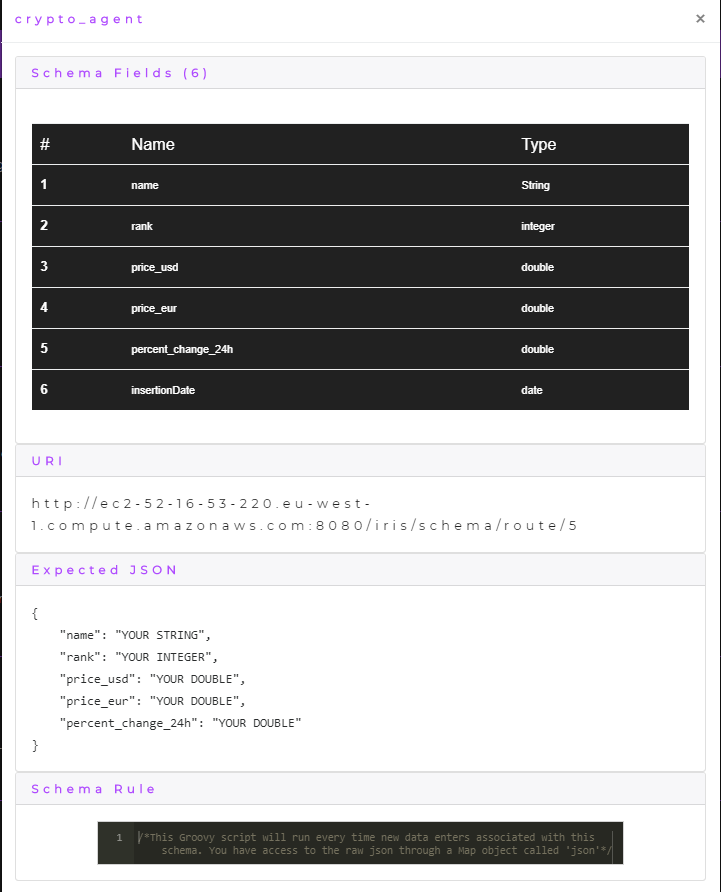
\includegraphics[width=\textwidth,height=\textheight,keepaspectratio]{iris-crypto-schema}
\end{center}
A screenshot of the Raspberry Pi agent schema in Iris.
\end{tcolorbox}
\caption{Raspberry Pi agent schema in Iris.}
\end{figure}

%Iris Raspberry Pi agent dashboard screenshot
\begin{figure}[H]
\begin{tcolorbox}
\begin{center}
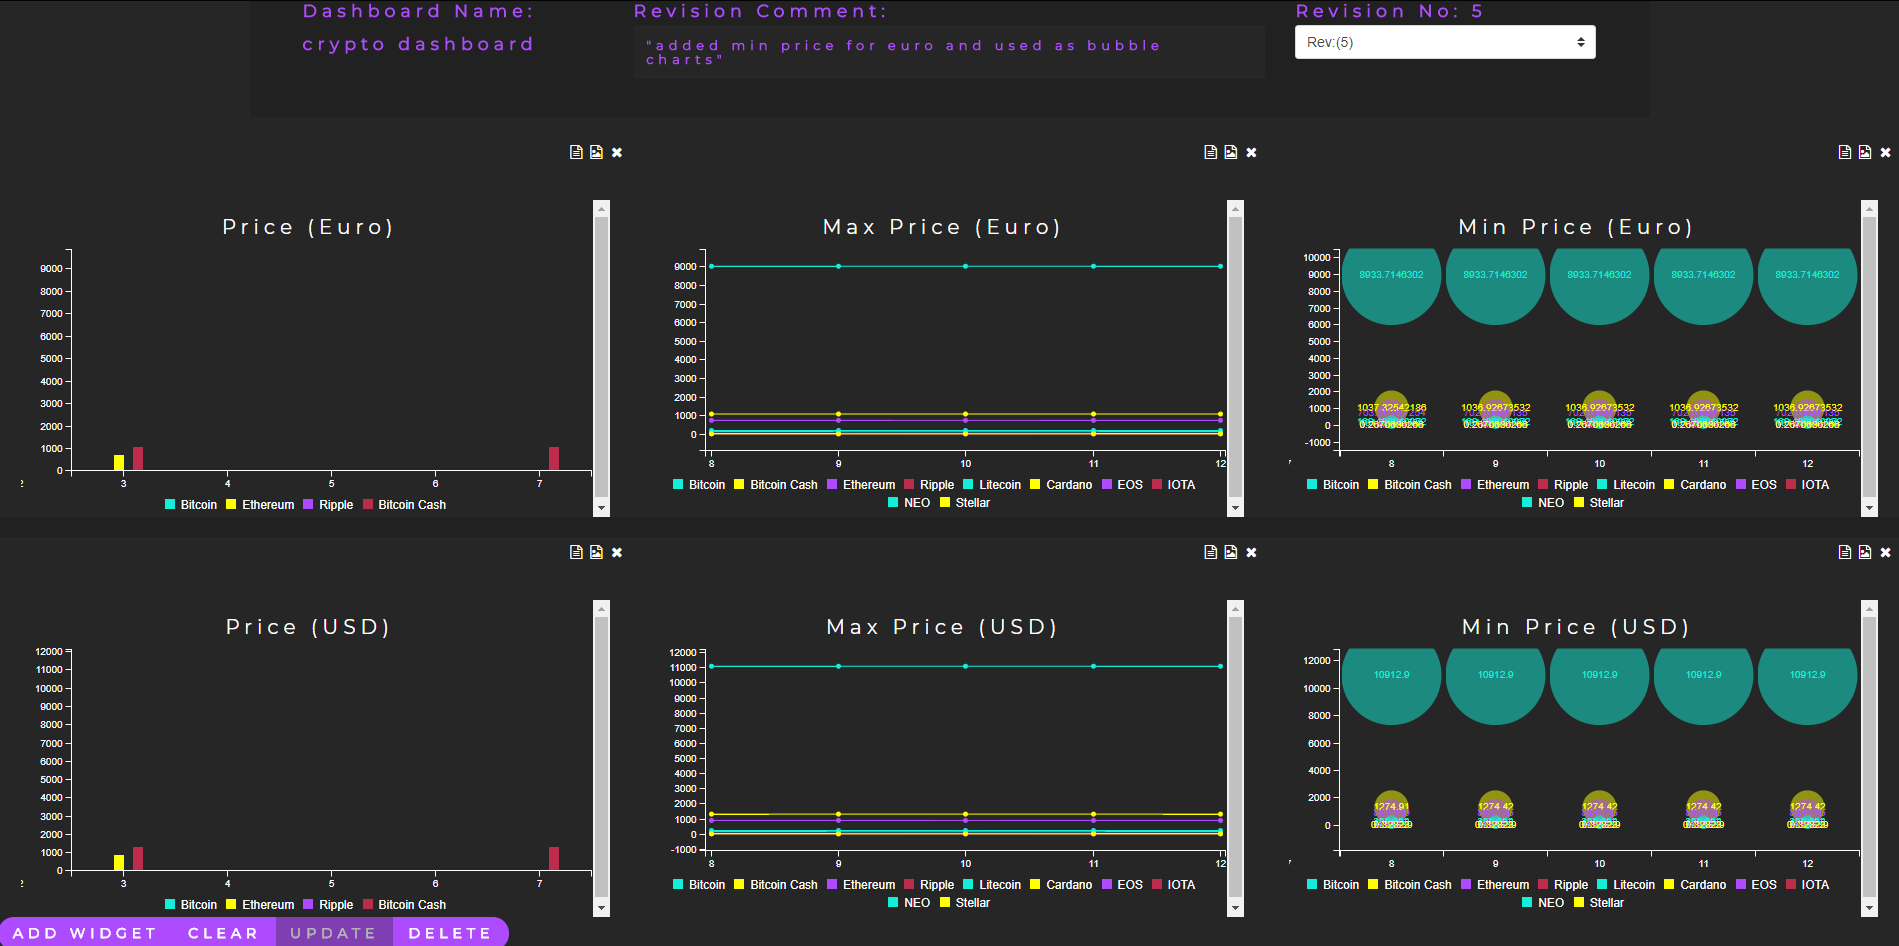
\includegraphics[width=\textwidth,height=\textheight,keepaspectratio]{iris-crypto-agent-dashboard}
\end{center}
A screenshot of the Raspberry Pi agent dashboard in Iris monitoring crypto currencies.
\end{tcolorbox}
\caption{Raspberry Pi agent dashboard in Iris.}
\end{figure}

\subsection{Node.js}
The Node.js agent shows how Iris can integrate with one of the most popular server-side frameworks and how it can monitor the status of the system running Node.js through the npm (node package manager) package `systeminformation'.

\subsubsection{Description}
Due to Node.js' rise in popularity in recent years this agent demonstrates how Iris can easily monitor a system using the `systeminformation' package from npm. The `systeminformation' package offers various levels of detail about the system running Node. Iris' schema for the Node.js agent measures the following attributes:
\begin{itemize}
    \item Operating System Name
    \item Current Uptime of the Operating System
    \item Current CPU Speed
    \item Total Memory Available
    \item Total Memory Free
    \item Total Memory Used
    \item Current CPU Load
\end{itemize}
A full list of all the obtainable attributes through `systeminformation' can be found here \url{https://github.com/sebhildebrandt/systeminformation}.

An important thing to note about this agent is that it takes use of Iris' ability to transform incoming data through scripting. Many of the memory attributes retrieved from `systeminformation' are represented in bytes, this agent uses Iris' centralised transformation abilities to transform the `memFree' attribute to be represented as gigabytes rather than bytes. This script also transforms all the `osName' attributes to be uppercase. Transforming these attributes in Iris through scripting removed the need for a redeployment of the Node.js application.

%Node.js agent transformation script
\begin{figure}[H]
\begin{tcolorbox}
\begin{center}
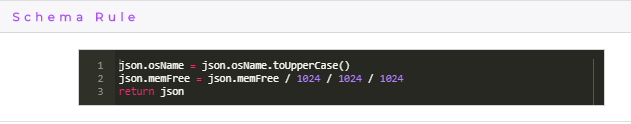
\includegraphics[width=\textwidth,height=\textheight,keepaspectratio]{node-transformation-script}
\end{center}
The transformation script for the Node.js agent which turns the `osName' attribute to uppercase and the `memFree' attribute to be gigabytes rather than bytes.
\end{tcolorbox}
\caption{Node.js agent transformation script.}
\end{figure}

\subsubsection{Linkage with Iris}
The Node.js agent is linked to Iris through a unique REST endpoint specific to the Node.js agent schema. All of the data being sent from the Node.js agent is sent to this endpoint. Once the data enters Iris, Iris will run through it's logic for checking for dashboards and charts associated with the schema and send the data through to the charts. 
%Add a ref to a section where you explain what iris does, so you dont have to keep repeating this for all agents
In this case Iris is monitoring raw data on three charts that are monitoring the current memory free in gigabytes, the current memory used and the current uptime of the system. The other charts display the max memory used over all operating systems and the pie chart shows all the types of operating systems which have run the agent, both of these use Elasticsearch aggregations to calculate the data for the charts.

%Node.js agent schema screenshot in Iris
\begin{figure}[H]
\begin{tcolorbox}
\begin{center}
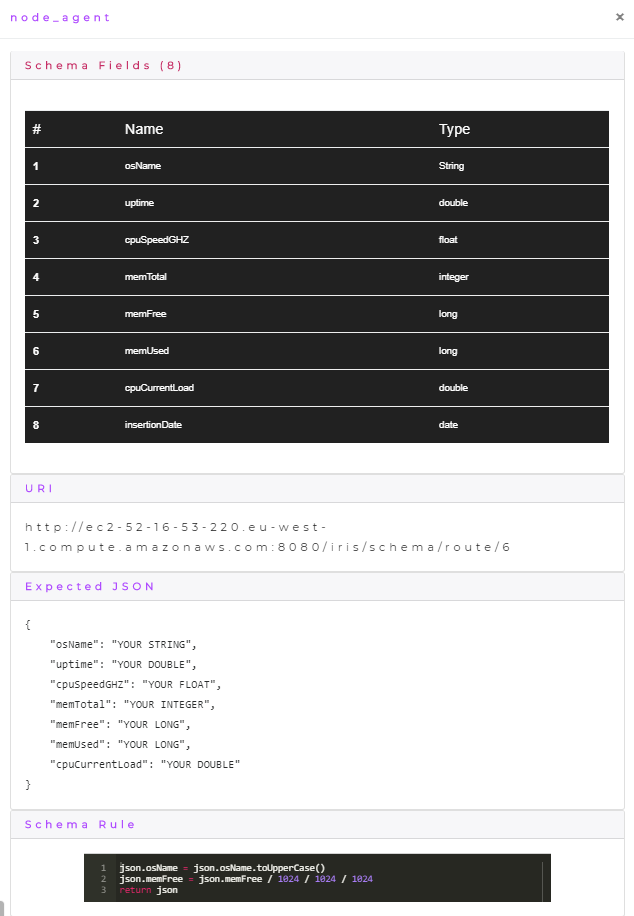
\includegraphics[width=\textwidth,height=\textheight,keepaspectratio]{iris-node-schema}
\end{center}
A screenshot of the Node.js agent schema in Iris.
\end{tcolorbox}
\caption{Node.js agent schema in Iris.}
\end{figure}

%Iris Node agent dashboard screenshot
\begin{figure}[H]
\begin{tcolorbox}
\begin{center}
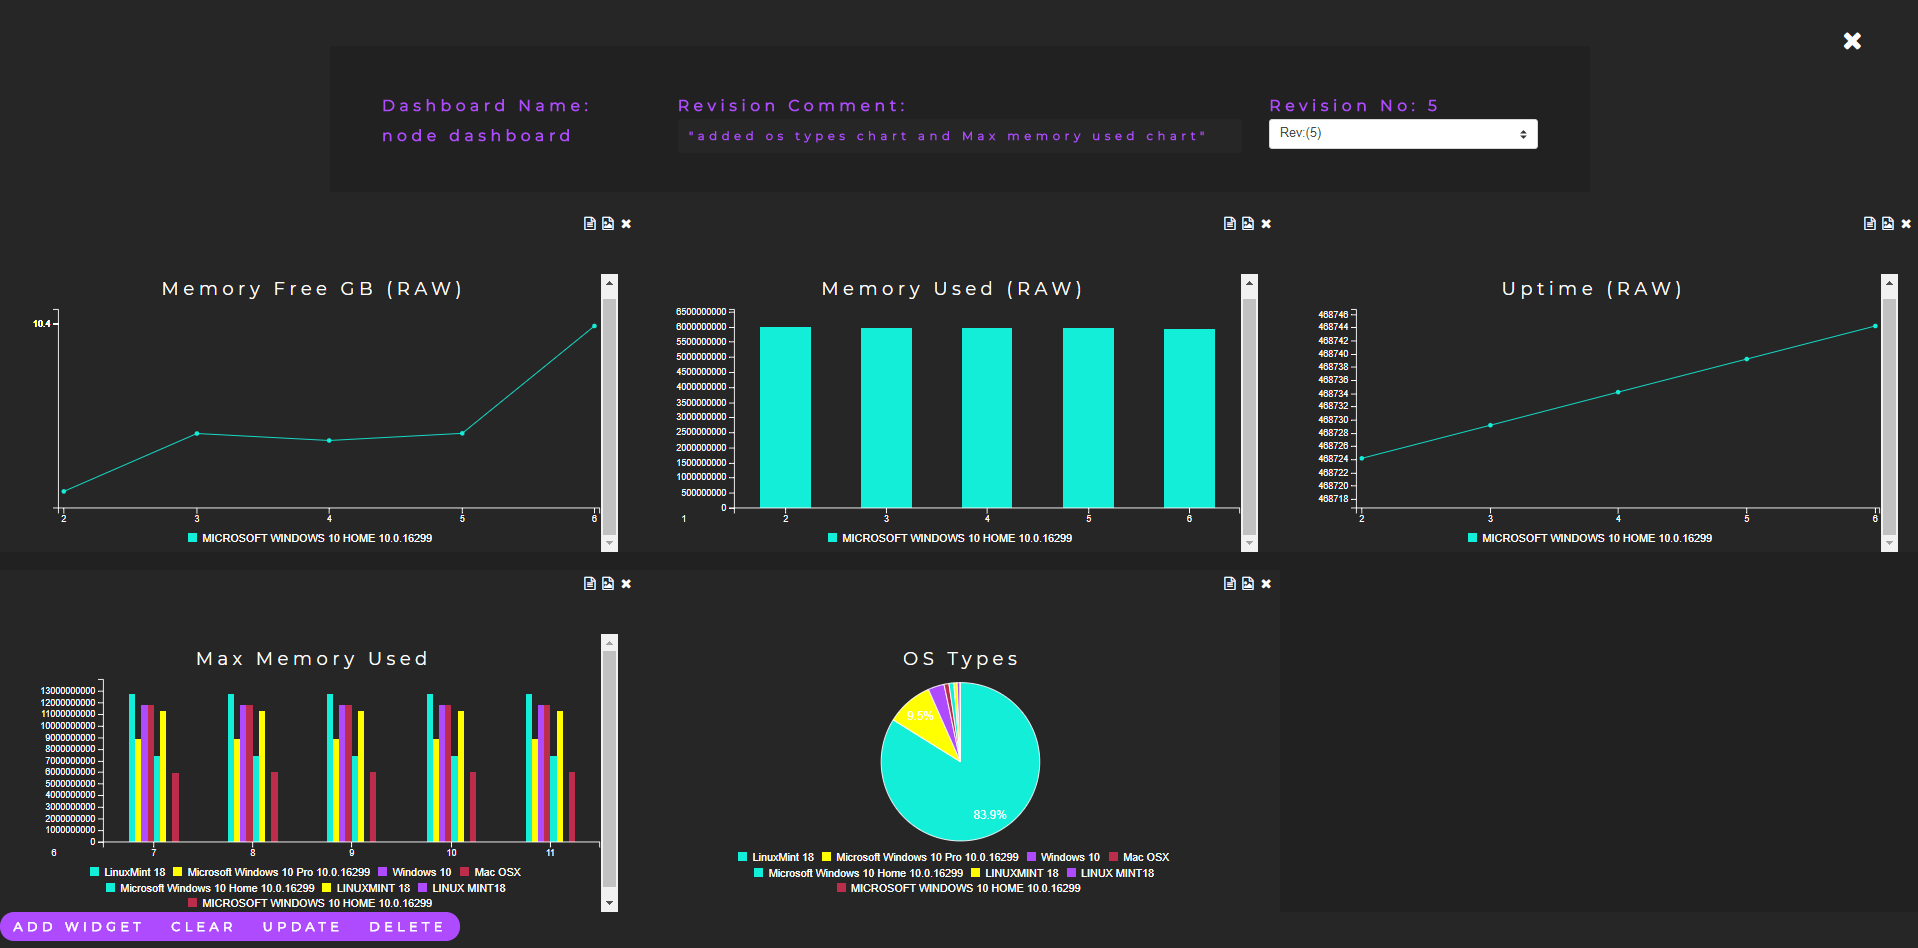
\includegraphics[width=\textwidth,height=\textheight,keepaspectratio]{iris-node-agent-dashboard}
\end{center}
A screenshot of the Node.js agent dashboard in Iris monitoring system information.
\end{tcolorbox}
\caption{Node.js agent dashboard in Iris.}
\end{figure}


\subsection{Selenium}
The Selenium agent demonstrates the versatility of Iris by monitoring the price of a guitar by scraping music store websites and monitoring the price of the guitar. This agent focuses on versatility over complexity.
\subsubsection{Description}
The Selenium agent demonstrates Iris' versatility through the Selenium web driver which is commonly used for web automation and functional testing. In this case Selenium is used in conjunction with a Selenium wrapper called `Selenide' to automate the scraping of music store websites for a specific guitar. On each site the guitar's price is taken from the webpage as well as the name of the music store, the price of the guitar and the name of the music store is then sent to Iris so that it may be monitored.

For more information on Selenide see their site here \url{http://selenide.org/}

\subsubsection{Linkage with Iris}
The Selenium agent is linked to Iris through a unique REST endpoint specific to the Selenium agent schema. All of the data being sent from the Selenium agent is sent to this endpoint. Once the data enters Iris, Iris will run through it's logic for checking for dashboards and charts associated with the schema and send the data through to the charts. 
%Add a ref to a section where you explain what iris does, so you dont have to keep repeating this for all agents
In this case Iris is monitoring raw data on a bar chart. The bar chart monitors the price of the guitar in euro and labels the chart based on the music store website that the price has been scraped from. In this case two sites have been scraped `Thomann' and `MusicStore.de', both sites are competitors and this reflects in the chart as both sites have matched the price of the guitar at the same price.

%Iris selenium agent schema screenshot
\begin{figure}[H]
\begin{tcolorbox}
\begin{center}
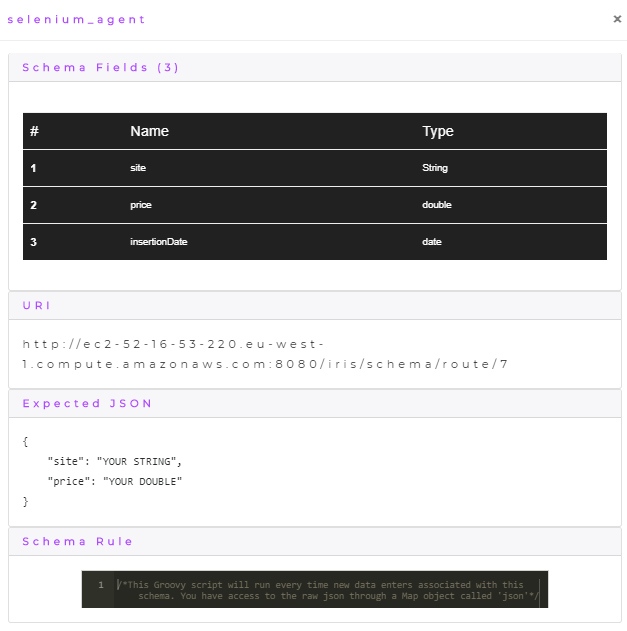
\includegraphics[width=\textwidth,height=\textheight,keepaspectratio]{iris-selenium-schema}
\end{center}
A screenshot of the Selenium agent schema in Iris.
\end{tcolorbox}
\caption{Selenium agent schema in Iris.}
\end{figure}

%Iris selenium agent dashboard screenshot
\begin{figure}[H]
\begin{tcolorbox}
\begin{center}
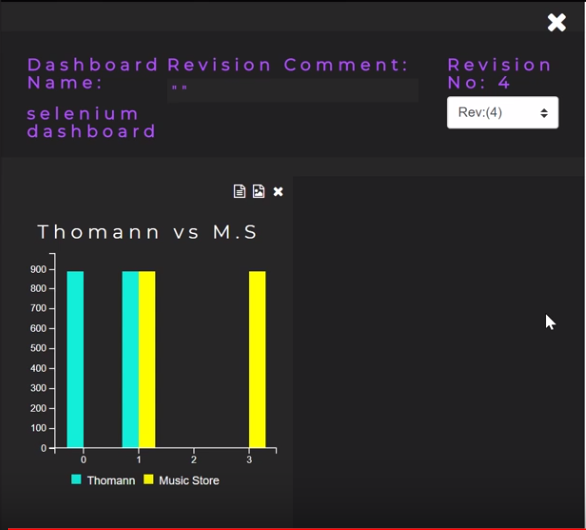
\includegraphics[width=\textwidth,height=\textheight,keepaspectratio]{iris-selenium-dashboard}
\end{center}
A screenshot of the Selenium agent dashboard in Iris.
\end{tcolorbox}
\caption{Selenium agent dashboard in Iris.}
\end{figure}

\subsection{MySQL}
The MySQL agent demonstrates how a user can monitor their database by converting the MySQL `information\_schema' results into JSON and sending them to Iris.
\subsubsection{Description}
The MySQL agent is significant for Iris as this agent was the inspiration for Iris in the beginning, as Onaware developers wanted a way to monitor a remote MySQL database with scripts and be able to monitor the database memory locally with a web application. The MySQL agent is a simple python script that connects to the MySQL instance and monitors all the databases as well as the amount of memory they use. The database name and the amount of memory it currently uses is then sent to Iris to be monitored. The python script is run every day at 8:00pm on the same AWS server that Iris is running on using a cron job.

%MYSQL statement script
\begin{figure}[H]
\begin{tcolorbox}
\begin{minted}{mysql}
SELECT table_schema AS "databaseName", 
ROUND(SUM(data_length + index_length) / 1024 /  1024, 2) as "memoryMB" 
FROM information_schema.TABLES 
GROUP BY table_schema;
\end{minted}
\end{tcolorbox}
\caption{MySQL Agent, MySQL `information\_schema' table query used in iris-mysql.py source code.}
\end{figure}

More information on the MySQL `information\_schema' table can be found here \url{https://dev.mysql.com/doc/refman/5.7/en/information-schema.html}


\subsubsection{Linkage with Iris}
The MySQL agent is linked to Iris through a unique REST endpoint specific to the MySQL agent schema. All of the data being sent from the MySQL agent is sent to this endpoint. Once the data enters Iris, Iris will run through it's logic for checking for dashboards and charts associated with the schema and send the data through to the charts. 
%Add a ref to a section where you explain what iris does, so you dont have to keep repeating this for all agents
The MySQL agent dashboard monitors the average memory taken up by each database in the MySQL instance and displays the results as a line chart in Iris.
%Iris mysql schema screenshot
\begin{figure}[H]
\begin{tcolorbox}
\begin{center}
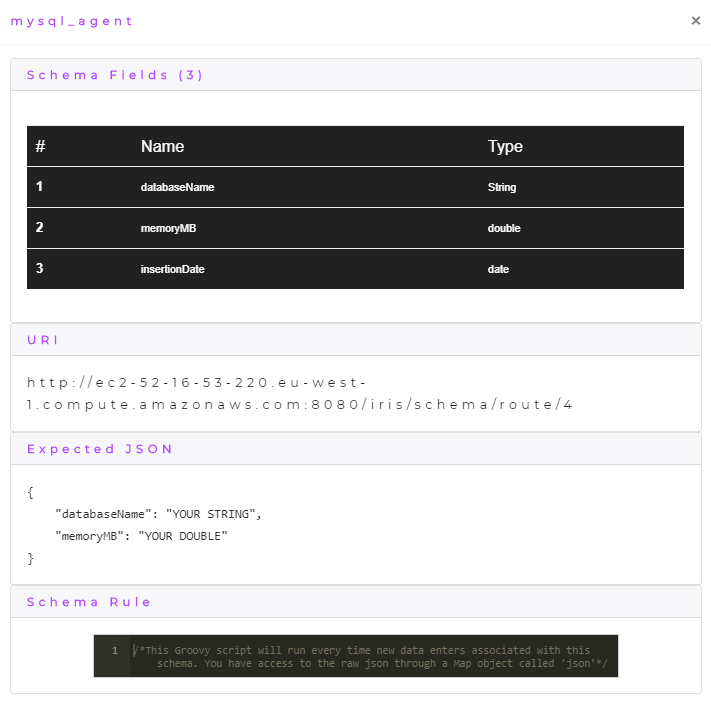
\includegraphics[width=\textwidth,height=\textheight,keepaspectratio]{iris-mysql-schema}
\end{center}
A screenshot of the MySQL agent schema in Iris.
\end{tcolorbox}
\caption{MySQL agent schema in Iris.}
\end{figure}

%Iris mysql dashboard screenshot
\begin{figure}[H]
\begin{tcolorbox}
\begin{center}
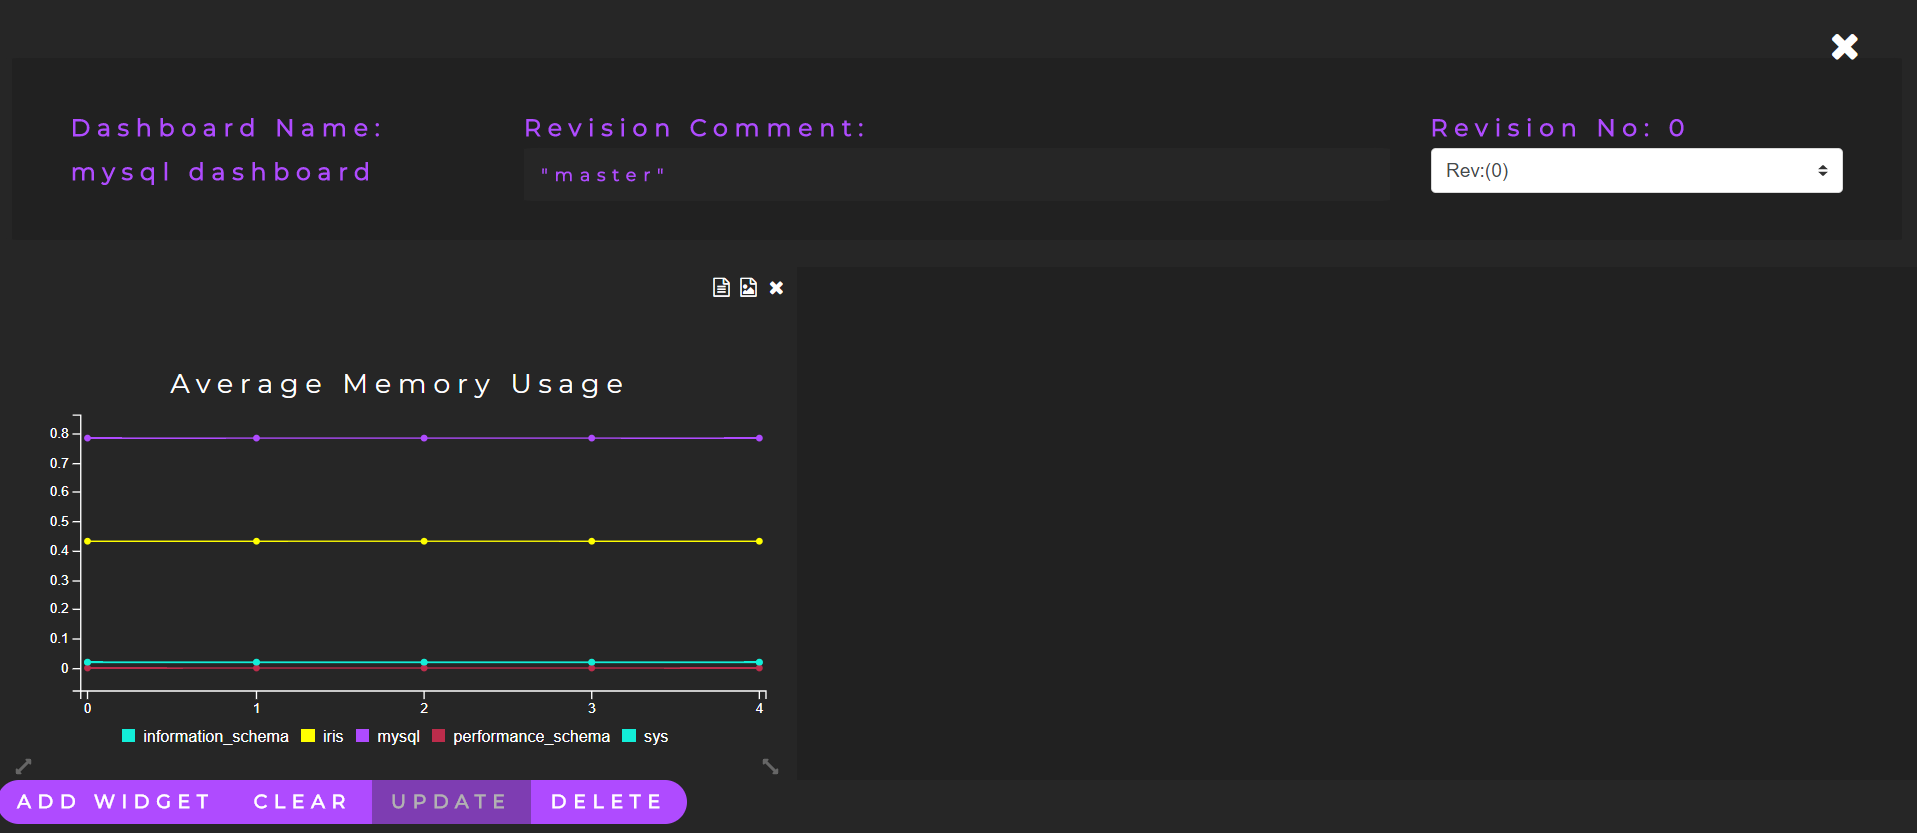
\includegraphics[width=\textwidth,height=\textheight,keepaspectratio]{iris-mysql-dashboard}
\end{center}
A screenshot of the MySQL agent dashboard in Iris.
\end{tcolorbox}
\caption{MySQL agent dashboard in Iris.}
\end{figure}

\chapter{Conclusions}
\section{Current Application State}
Currently Iris is in a stable state and has achieved what it was designed to do dynamic data monitoring. In the Semester 1 report the design and features of the Iris core framework are discussed in regards to schemas, dashboards and Iris' use of Elasticsearch. All of these features were implemented successfully and collaborate to deliver a fully dynamic data monitoring implementation.

Iris demonstrates its capabilities in live production on AWS where it monitors data from several data sources which are active on different platforms and push of different forms of data to Iris. Iris handles setting up an application schema for the data sources and handles the incoming data being pushed from these data sources. Iris allows users to track their data through dashboards and Elasticsearch aggregations in realtime which helps verify Iris' current state in this lifecycle.

\section{Future Development}
The goal of this lifecycle was to implement the core framework of Iris which Onaware could work with and expand upon. Throughout the development of Iris a potential features list has been growing within Onaware. Below is a summary of some of the features which are being considered for Iris:
\begin{itemize}
    \item Storing unmodified data. Currently when a user writes a transformation script to transform the data, the transformed data is being stored in Elasticsearch. It would be better to store the raw unmodified data as well as the modified data.
    \item Replace Elasticsearch Aggregation terminology with more user friendly terminology, making it easier for anyone to build Elasticsearch aggregations.
    \item Add a State Disc Chart list. This would be a list of state disc charts inside one widget.
    \item Add a dashboard widget which simply displays text, this can be useful for dumping programming exceptions or to send log file contents into a widget on a dashboard.
    \item Chart merging. Allow a user to merge two or more charts to aid their data visualisation.
    \item Create a dedicated area for downloading and uploading common applications for pushing data to Iris, this would be similar to a marketplace.
\end{itemize}
The features listed above will be discussed in more detail with Onaware once Iris starts its new lifecycle within Onaware.

\section{Alternative Approaches}
The main alternative approach which was discussed for building Iris was the idea of using Node.js rather than Grails 3.

Iris was built using Grails, a technology which appears to losing popularity as a means for building web applications. This became evident relatively quickly in the research stage of Iris as there was difficulty finding appropriate plugins and libraries for Grails 3 (the newest release of Grails) that are essential for Iris. The reason Grails 3 is being discussed and not its prior releases is because it shows how Grails is beginning to decline in popularity. For example there is 1,255 plugins for Grails versions 1\&2, but currently there is only 239 plugins for Grails 3, which can be seen here \url{http://plugins.grails.org/}. Due to the lack of community support for Grails 3, using a different technology such as Node.js would have benefited Iris. Node.js which uses the `npm' package manager contains over 650,000 packages \parencite{ModuleCounts}. This would have increased the development time of Iris dramatically as a lot of Iris' code had to be written from scratch, and could have benefited from reusing code from the npm package manager.

Another reason for considering Node.js for Iris, was due to Iris needing to monitor data in realtime. Although Iris currently doesn't struggle with this operation, Node.js' I/O architecture is designed to be non-blocking, which allows requests to be dealt with asynchronously, meaning Iris can handle incoming data requests asynchronously.

Another reason for considering Node.js for Iris is the fact that the majority of requests sent from the client to Iris are in the form of JSON. Once the JSON request is recieved by Iris it needs to be parsed into Groovy code. Groovy has made excellent libraries for parsing JSON but it would be more ideal if possible to work with the same languages both frontend and backend if possible. Node.js makes this possible by having the server code in javascript.

Lastly, Iris could benefit from using a more efficient way of dealing with DOM manipulation, jQuery is an older technology and is now starting to be replaced by frontend frameworks. Using a frontend framework such as React.js would allow Iris to render dashboard charts more efficiently due to its use of a virtual DOM, as well as bind the DOM data to javascript variables. React.js also uses components which add a great increase in reusability and testability for the frontend. All React.js code is written in javascript meaning the server and client can communicate in the same language if Node.js was being used for the server code. Using a frontend framework allows the frontend and backend of a project to remain loosely coupled making them both easier to work on.

%No cite prints all references even if they are not in the document!!
% \nocite{*}
\printbibliography

%%%%%%%%%%%%%%%%%%%%%%%%%%%%%%%%
\clearpage

\begin{appendices}


\chapter{Overview of Code Repository}
All of the code developed in this project is available on bitbucket. Following common conventions a separate repository is used for Iris and for each of the separate agents. They can all be found at the following urls:
\begin{itemize}
    \item Iris (Core) - \url{https://bitbucket.org/DeanGaffney/iris}.
    \item Iris-Selenium - \url{https://bitbucket.org/DeanGaffney/iris-selenium}.
    \item Iris-Raspberry Pi - \url{https://bitbucket.org/DeanGaffney/iris-crypto-rates}.
    \item Iris-MySQL - \url{https://bitbucket.org/DeanGaffney/iris-mysql}.
    \item Iris-Android - \url{https://bitbucket.org/DeanGaffney/iris-android}.
    \item Iris-Node.js - \url{https://bitbucket.org/DeanGaffney/iris-node}.
\end{itemize}

Due to the amount of code developed it is impractical to include the code within this report. This overview will be limited to a high level summary. \Cref{fig:cloc} gives a breakdown of code by language using the cloc utility. Third party code was excluded from this count. Since the various components of the systems were developed using different languages the breakdown by language closely follows the breakdown by component.

\begin{figure}[H]
\begin{tcolorbox}
\begin{center}
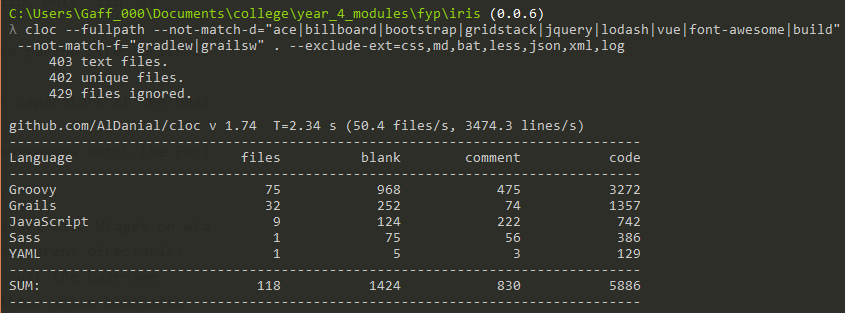
\includegraphics[width=\textwidth,height=\textheight,keepaspectratio]{iris-cloc}
\end{center}
A screenshot of the cloc utility run on Iris, the command filters all third party code and only counts the lines of code in Iris.
\end{tcolorbox}
\caption{Cloc results.}
\label{fig:cloc}
\end{figure}

The breakdown shown in \cref{table:component:breakdown} closely follows the separate components of the system.
\begin{table}[H]
\centering
\small
\setlength\tabcolsep{10pt}
 \begin{tabular}{ccrr}
 \hline
 \multicolumn{2}{l}{\bfseries Component/Language}
& \bfseries Files & \bfseries Line Count\\
 \hline\hline
 \multicolumn{2}{l}{\bfseries\smaller Schemas}\\
  & Groovy & 10 & 461\\ 
  & Grails & 5 & 169\\
  \multicolumn{2}{l}{\bfseries\smaller Dashboards}\\
   & Groovy & 3 & 292\\
  & Grails & 9 & 427\\
  & Javascript & 1 & 191\\
  \multicolumn{2}{l}{\bfseries\smaller Charts} \\
  & Groovy & 2 & 128\\
  & Javascript & 4 & 308\\
  \multicolumn{2}{l}{\bfseries\smaller Elasticsearch} \\
  & Grails & 3 & 169\\
  & Groovy & 6 & 245\\
  & Javascript & 2 & 110\\
  \multicolumn{2}{l}{\bfseries\smaller Integration Tests} \\
  & Groovy & 14 & 761\\ 
  \multicolumn{2}{l}{\bfseries\smaller Unit Tests}\\
   & Groovy & 13 & 668\\ 
  \multicolumn{2}{l}{\bfseries\smaller Utilities}\\
   & Groovy & 18 & 384\\ 
  \multicolumn{2}{l}{\bfseries\smaller Other Services} \\
  & Groovy & N/A & 1573\\ 
\end{tabular}
\caption{Summary of component lines of code.}
\label{table:component:breakdown}
\end{table}

\import{.}{trello}

\end{appendices}

\end{document}
